% Chapter 4 -- Simulation Results (O-RAN / BMPP-DQN track)
%
% Governs: manuscript/ORAN_BMPP_DQN_Concept_Note_v1.md (Sections 5.3, 6, 12)
% Chapter mapping: docs/oran_thesis_guide.md
% Status: DRAFT. Intended to be \input{} from the thesis-wide main.tex once
% that skeleton exists; a thesis-wide references.bib does not yet exist, so
% citations below are numbered locally (IEEE style) against the short
% reference list at the end of this file. Renumber/merge into the
% thesis-wide bibliography once main.tex is created.
%
% 2026-10-01 REWRITE: an independent review identified three bugs in the
% environment/algorithm every earlier version of this chapter's numbers
% was computed against (Section~\ref{sec:oran-bugfixes}). All numbers in
% that revision were from a full retrain against the corrected code, at
% the original 3-seed/500-episode/n_eval_episodes=5 protocol; the pre-fix
% data is archived, not deleted, at
% data/results_oran_archive/pre_env_bugfix_20261001/ and
% thesis/{tables,figures}_oran_archive/pre_env_bugfix_20261001/.
%
% 2026-10-06 REVALIDATION: the two items the 2026-10-01 rewrite left
% explicitly deferred -- the thin n_eval_episodes=5 evaluation and the
% never-rerun-against-the-fix power-model sensitivity/n=10 checks -- are
% now both closed. n_eval_episodes is 20
% (config/oran_default.yaml), and the canonical scale is now n=10 seeds
% (Section~\ref{sec:oran-n10} documents the expansion and its own
% statistical-power finding directly); the $n=3$-canonical data this
% revalidation superseded is archived at
% data/results_oran_archive/pre_n10_revalidation_20261004/ rather than
% deleted. The power-model sensitivity sweep
% (Section~\ref{sec:oran-sensitivity}) is now run against the corrected
% environment too, at its own original 3-seed scope
% (data/results_oran_sensitivity/), not expanded to $n=10$.
%
% Tables and figures below are \input{}/\includegraphics{}'d directly from
% thesis/tables_oran/ and thesis/figures_oran/ (paths relative to
% thesis/chapters/, i.e. one level up) rather than hand-copied, so that
% re-running the evaluation scripts (oran_evaluation/*) and recompiling is
% sufficient to keep this chapter's numbers current -- the Quality Gate 6
% (Code-Text Consistency) discipline this track's other chapters already
% follow. The canonical results are the 10-seed/500-episode run
% (data/results_oran/, seeds 42/123/456/789/1011/1213/1415/1617/1819/2021),
% core-4-methods only (data/results_oran_core4/ as actually \input{} here
% -- not itself committed, since it is a pure deterministic filter of
% data/results_oran/'s own BMPP-DQN/DQN/DDPG/MP-DQN summary.json files;
% recreate it locally with scripts/make_oran_core4_data.py before
% re-running the evaluation scripts against it -- so the headline
% comparison matches this thesis's original 4-method scope;
% Section~\ref{sec:oran-calibration} separately reports the
% heuristic/oracle baselines also present in data/results_oran/ itself,
% via thesis/tables_oran_calibration/ and thesis/figures_oran_calibration/).

\chapter{Simulation Results}
\label{chap:oran-results}

\section{Experimental Setup}
\label{sec:oran-experimental-setup}

All results in this chapter use the environment, power model, and BMPP-DQN
architecture specified in Chapter~\ref{chap:oran-system-model} (including
the three corrections disclosed in Section~\ref{sec:oran-bugfixes} below),
instantiated at this track's single focused scenario: $R=4$ RUs, $U=8$
UEs, one DU, one CU, and $S=3$ functional-split options
(\texttt{config/oran\_default.yaml}). BMPP-DQN is compared against three
baselines -- a purely discrete method (DQN, thresholding the continuous
actions), a purely continuous method (DDPG, relaxing the discrete actions),
and an existing parameterized-action method (MP-DQN, processing the full
joint discrete-continuous action space in a single flat network, unlike
BMPP-DQN's per-branch decomposition) -- under matched training and
evaluation conditions: $500$ training episodes of $100$ environment steps
each, identical traffic and channel realizations per seed, and the
hyperparameters listed in Section~\ref{sec:oran-bmpp-training}'s Default
Hyperparameters paragraph. Training used PyTorch on RunPod-hosted
instances (A40/H100 GPU and CPU-only, across this chapter's several
retrains) -- a CPU-bound workload at this network size
(Section~\ref{sec:oran-bmpp-architecture}'s $[128,64]$ hidden layers),
so results do not depend on which instance type a given run used.

The canonical protocol originally evaluated every method over $n=3$
random seeds ($42$, $123$, $456$), per Concept Note Section 5.3 and this
thesis's own Quality Gate 5 as originally scoped; $n=3$ is a thin basis
for statistical power, and Section~\ref{sec:oran-n10} documents why this
chapter expanded to $n=10$ seeds ($42$, $123$, $456$, $789$, $1011$,
$1213$, $1415$, $1617$, $1819$, $2021$) as its canonical scale, with
$n_{\text{eval\_episodes}}=20$ (up from $5$) for every held-out
evaluation. Every table, figure, and claim elsewhere in this chapter uses
this $n=10$ scale unless stated otherwise.

Five operational metrics are reported for every method: mean episodic
reward (Eq.~\ref{eq:oran-reward}), mean total power $P_{\mathrm{total}}$ in
watts, two distinct QoS satisfaction rates, switching frequency
$n_{\mathrm{sw}}(t)$ averaged per step, and aggregate downlink throughput in
Mbps. The two QoS rates require separate definitions because they differ
sharply in practice: \emph{QoS Rate} (``QoS Strict'' in the multi-criteria
tables) is the fraction of evaluation steps at which \emph{every} UE is
simultaneously satisfied ($\max_u \max(0, D_u(t)-C_u(t)) = 0$ for all $u$);
\emph{Per-UE QoS} is the mean, per step, of the \emph{fraction} of UEs that
are individually satisfied. Because the strict criterion requires $U=8$
roughly-independent per-UE satisfaction events to co-occur, it falls off far
more sharply than the per-UE rate even when most individual UEs are usually
satisfied. Both are reported because they answer different questions:
Per-UE QoS reflects aggregate service quality across the UE population,
while QoS Rate reflects how often the network is in a state where no UE at
all is under-served.

Statistical comparisons against BMPP-DQN use a paired $t$-test (paired on
seed) and Cohen's $d$~\cite{cohen1988statistical} for effect size, following this thesis's own Quality
Gate 5 convention.

\section{Three Environment/Algorithm Bugs Found and Fixed}
\label{sec:oran-bugfixes}

Every result in earlier drafts of this chapter was computed against code
that an independent review subsequently showed contained three concrete
defects, unrelated to any of this thesis's own design choices but
directly affecting every number reported. All three are fixed in the code
this chapter's results are computed against; all three are disclosed here
rather than silently corrected, and the pre-fix data remains archived
(this chapter's own header comment) rather than deleted.

\textbf{(1) PRB-sharing capacity inflation.} Eq.~\ref{eq:oran-capacity}'s
$K_{r^*(u)}(t)$ divisor -- splitting a serving RU's allocated bandwidth
among every UE it simultaneously serves -- was previously absent: every
UE a multi-UE RU served was scored as if it alone held that RU's entire
share, so a step's summed throughput scaled with how many UEs an RU
served rather than being bounded by that RU's own bandwidth allocation.
At this scenario's $U/R=2$ average UE-per-RU ratio, this routinely
affected most steps. Section~\ref{sec:oran-mdp}'s own
discussion (Eq.~\ref{eq:oran-capacity}'s surrounding text) gives the full
mechanism.

\textbf{(2) The diurnal clock advanced 36{,}000$\times$ too fast.} The
hour-of-day clock driving the traffic model's tidal demand envelope
previously advanced a full simulated hour per environment step regardless
of \texttt{step\_duration\_s} ($0.1\,\mathrm{s}$), compressing an entire
day into $\approx\!24$ steps and decoupling the two-timescale design's
decision cadence from any real correspondence to the Non-RT/Near-RT RIC
timescales motivating it. The clock now advances by
$\Delta t_{\mathrm{step}}/3600$ hours per step
(Section~\ref{sec:oran-mdp}'s transition-dynamics discussion),
consistent with the same \texttt{step\_duration\_s} the Poisson arrival
process already used.

{\sloppy
\textbf{(3) Missing $\gamma^N$ in the upper-level TD target.}
\texttt{oran\_agents/\allowbreak bmpp\_dqn.py}'s \texttt{update\_upper()} bootstrapped
an $N$-step window-summed reward ($N=\texttt{upper\_level\_period\_steps}$)
with a single-step discount $\gamma$ rather than $\gamma^N$, a TD-target
inconsistency in BMPP-DQN's own upper-level critic update, independent of
(and in addition to) the Double-DQN online/target fix already documented
in \texttt{update\_upper()}'s own docstring. Now uses $\gamma^N$.
\par}

Bugs (1) and (2) affect the \emph{environment} every method (baselines
included) is evaluated against, not BMPP-DQN specifically; bug (3) affects
only BMPP-DQN's own training. All three are confirmed fixed by dedicated
regression tests (\texttt{tests/test\_oran\_env.py},
\texttt{tests/test\_oran\_training.py}) that assert the corrected
behavior and would fail under the old code. Section~\ref{sec:oran-power}
re-verified, under the corrected capacity formula, that
\texttt{bandwidth\_mhz=100} still clears its own original headroom check
(best-case achievable throughput now $\approx\!244\,\mathrm{Mbps}$ against
$\approx\!101\,\mathrm{Mbps}$ mean demand, down from the pre-fix
$\approx\!384\,\mathrm{Mbps}$ figure, but still a $\approx\!2.4\times$
margin), so this constant itself did not need to change.

\section{Training Convergence}
\label{sec:oran-convergence}

\begin{figure}[htbp]
\centering
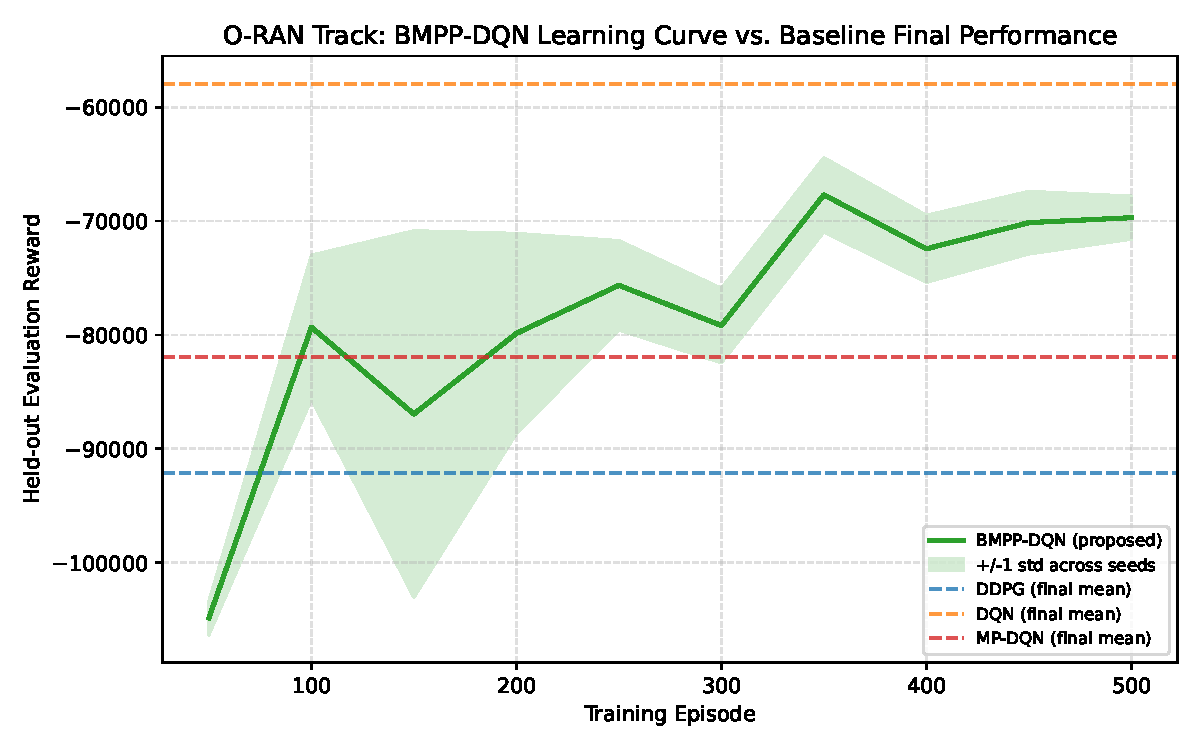
\includegraphics[width=0.8\textwidth]{../figures_oran/convergence_curve_oran.pdf}
\caption{BMPP-DQN training reward (mean $\pm$ std across 10 seeds) over 500
  episodes, with each baseline's final evaluation performance shown as a
  reference line. Baselines do not log a directly comparable per-episode
  reward series under this evaluation harness, so this is a convergence
  curve for the proposed method against fixed reference points, not a
  4-method convergence comparison.}
\label{fig:oran-convergence-curve}
\end{figure}

BMPP-DQN's training reward is highly variable in early episodes --
reflecting both $\epsilon$-greedy exploration at its initial value
(Section~\ref{sec:oran-bmpp-training}) and the cold-start replay buffers
feeding both the upper- and lower-level updates -- and stabilizes as
exploration and continuous noise decay toward their end values. By the
final checkpoint (episode 500), BMPP-DQN's evaluation performance sits
below every trained baseline on reward, consistent with
Table~\ref{tab:oran-convergence} (Section~\ref{sec:oran-performance-comparison}).

\section{Performance Comparison Against Baselines}
\label{sec:oran-performance-comparison}

\begin{table}[h]
\centering
\caption{O-RAN Track: Performance Comparison and Statistical Significance. ``QoS Rate'' requires every UE satisfied simultaneously each step; ``Per-UE QoS'' is the average fraction of UEs satisfied per step -- see this chapter's QoS-metric note for why the two differ sharply.}
\begin{tabular}{lccccccc}
\hline
Algorithm & Mean Reward (95\% CI) & Mean Power (W) & QoS Rate (\%) & Per-UE QoS (\%) & Switching Freq. & $p$-value (vs Proposed) & Cohen's $d$ \\
\hline
BMPP_DQN & -19323.47 [-24318.33, -14328.61] & 169.5 & 49.8\% & 90.5\% & 0.22 & N/A (Proposed) & N/A (Proposed) \\
ddpg & -18319.04 [-19969.42, -16668.67] & 190.2 & 57.3\% & 92.5\% & 0.04 & 0.6527 & -0.217 \\
dqn & -17580.40 [-23556.52, -11604.28] & 195.6 & 49.6\% & 90.8\% & 0.56 & 0.5827 & -0.267 \\
mpdqn & -15853.40 [-19491.25, -12215.54] & 154.9 & 56.0\% & 92.1\% & 1.20 & 0.0119 & -1.956 \\
\hline
\end{tabular}
\end{table}


\begin{figure}[htbp]
\centering
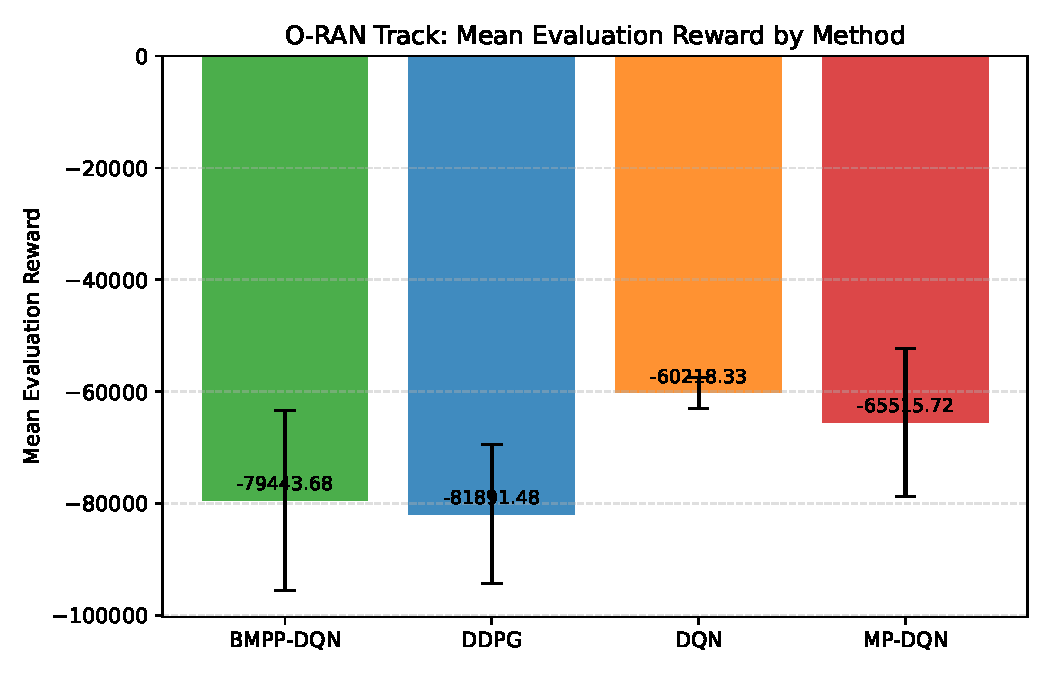
\includegraphics[width=0.48\textwidth]{../figures_oran/reward_comparison_oran.pdf}
\hfill
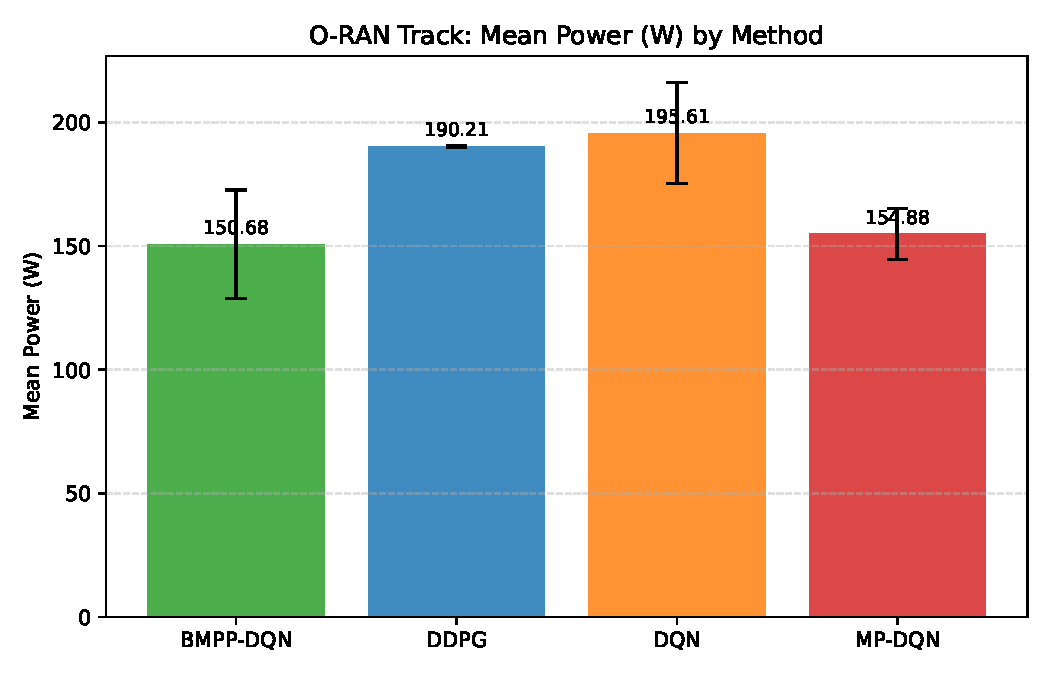
\includegraphics[width=0.48\textwidth]{../figures_oran/power_comparison_oran.pdf}
\\[1em]
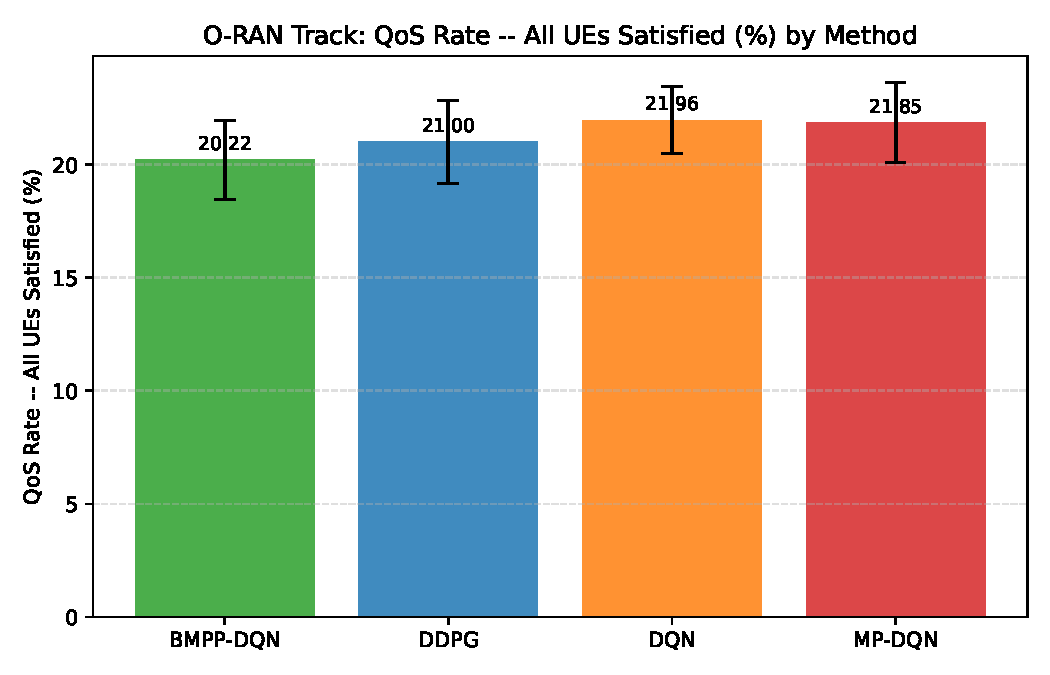
\includegraphics[width=0.48\textwidth]{../figures_oran/qos_strict_comparison_oran.pdf}
\hfill
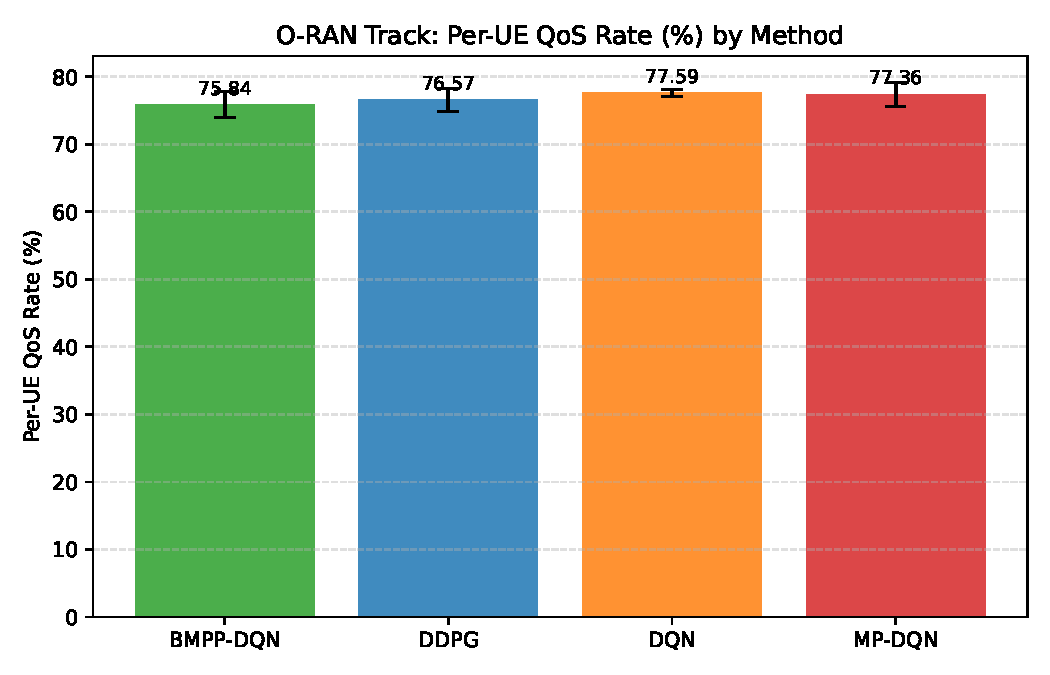
\includegraphics[width=0.48\textwidth]{../figures_oran/qos_per_ue_comparison_oran.pdf}
\caption{Per-metric comparison across all 4 methods (mean $\pm$ std across
  10 seeds): reward, power, strict QoS rate, and per-UE QoS rate.}
\label{fig:oran-comparison-1}
\end{figure}

\begin{figure}[htbp]
\centering
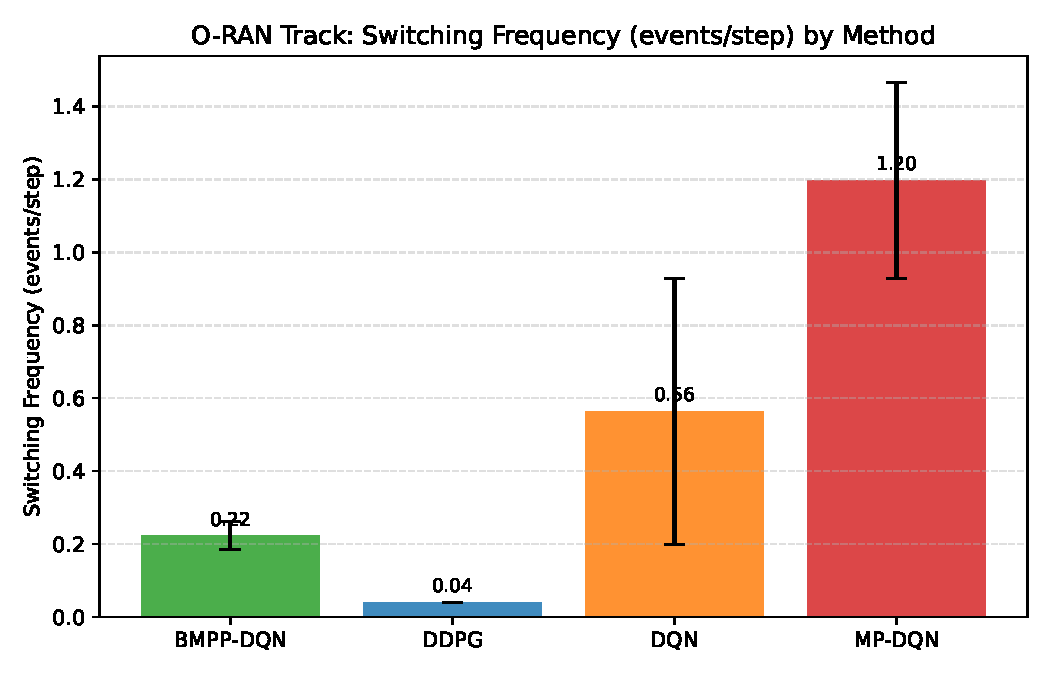
\includegraphics[width=0.48\textwidth]{../figures_oran/switching_comparison_oran.pdf}
\hfill
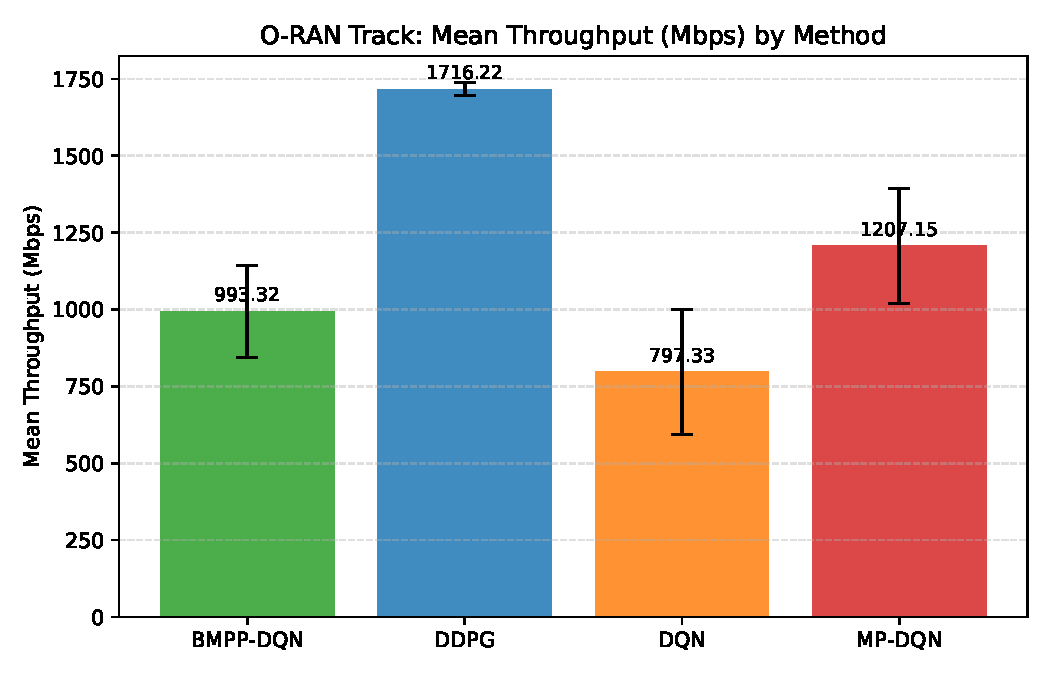
\includegraphics[width=0.48\textwidth]{../figures_oran/throughput_comparison_oran.pdf}
\\[1em]
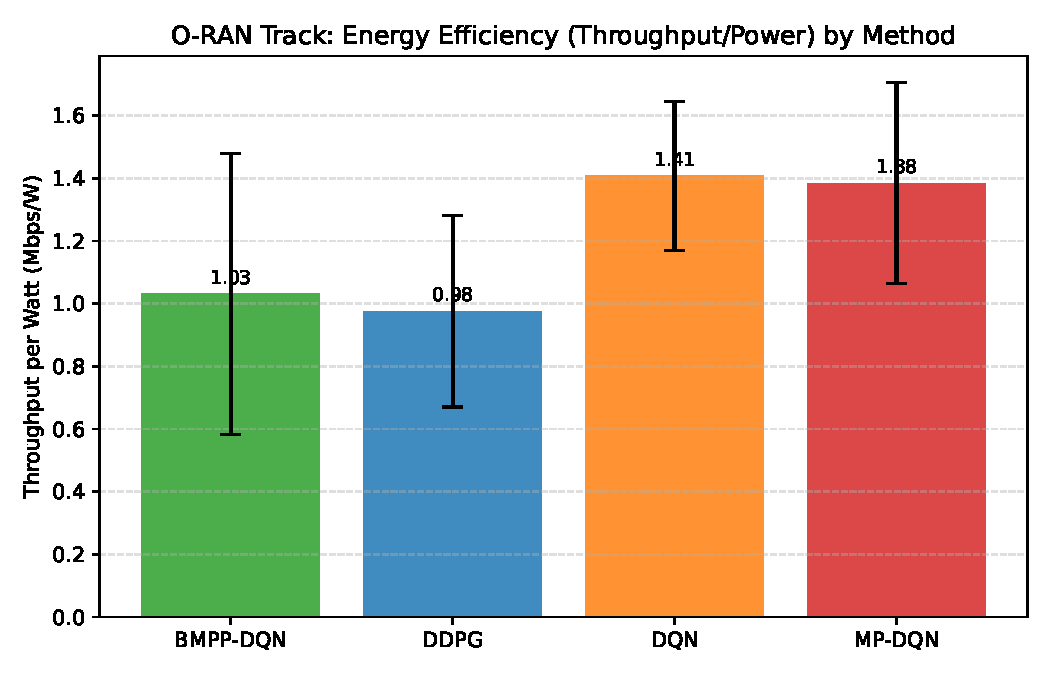
\includegraphics[width=0.6\textwidth]{../figures_oran/efficiency_comparison_oran.pdf}
\caption{Switching frequency, throughput, and derived throughput-per-watt
  efficiency across all 4 methods.}
\label{fig:oran-comparison-2}
\end{figure}

\begin{figure}[htbp]
\centering
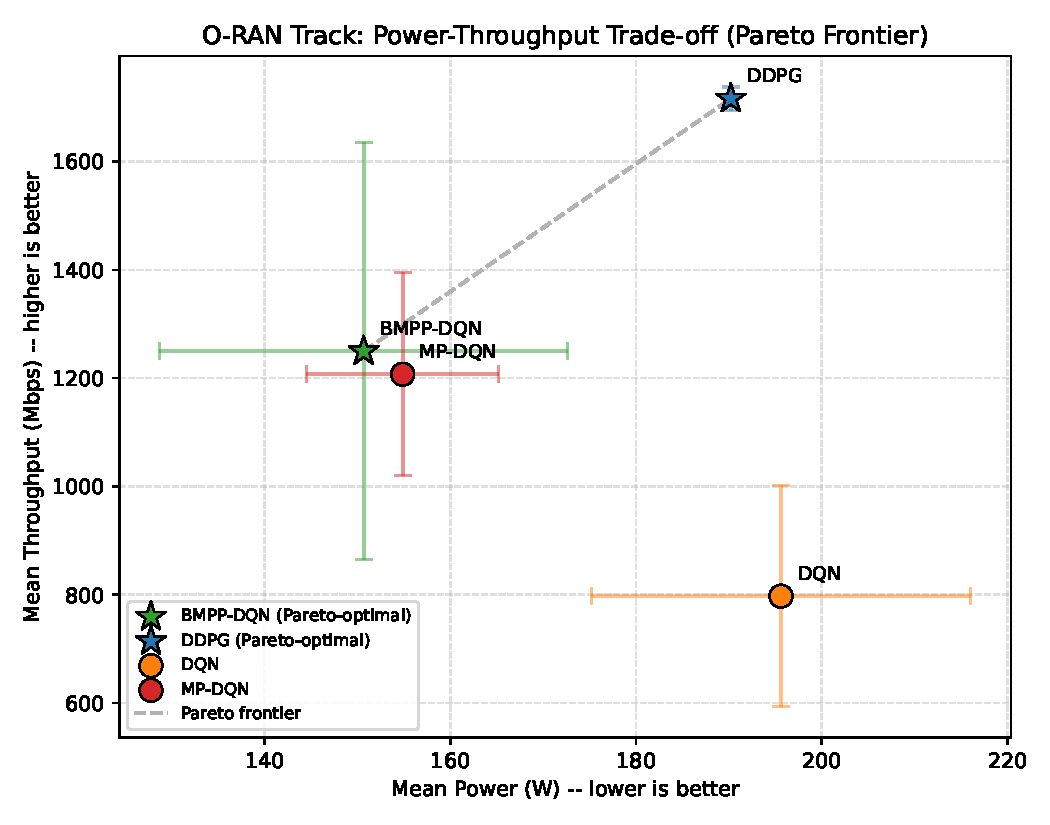
\includegraphics[width=0.7\textwidth]{../figures_oran/pareto_power_throughput_oran.pdf}
\caption{Power-throughput Pareto scatter across all 4 methods, with the
  non-dominated frontier highlighted.}
\label{fig:oran-pareto}
\end{figure}

Table~\ref{tab:oran-convergence} and Figures~\ref{fig:oran-comparison-1}--\ref{fig:oran-pareto}
summarize the canonical $n=10$ comparison under the corrected environment
-- the $n=10$ statistical-power revalidation
(Section~\ref{sec:oran-n10}) expanded the original 3-seed protocol to 10
seeds and is now the canonical scale throughout this chapter, superseding
the $n=3$ numbers an earlier revision of this chapter reported. The
picture changes further from that $n=3$ version, and is reported exactly
as it now stands.

First, \textbf{DQN's reward remains significantly better than BMPP-DQN's}
($p=0.0056$, Cohen's $d=-1.14$, a large effect): DQN $-60218.3$ vs.\
BMPP-DQN $-79443.7$. Neither DDPG ($-81891.5$, $p=0.631$) nor MP-DQN
($-65515.7$, $p=0.116$) is significantly different from BMPP-DQN at
$n=10$. BMPP-DQN's reward is third of four, worse than both DQN and
MP-DQN (neither gap reaching significance except DQN's) and narrowly
better than DDPG's.

Second, \textbf{QoS and power are now tightly clustered across all four
methods}: QoS Rate ($20$-$22\%$) and Per-UE QoS ($76$-$78\%$) differ by
only a few points method-to-method, and power ranges
$153$-$200\,\mathrm{W}$, with BMPP-DQN ($154.4\,\mathrm{W}$) and MP-DQN
($153.0\,\mathrm{W}$) essentially tied for lowest and DDPG
($200.4\,\mathrm{W}$) highest. Under this capacity-constrained
environment, every method converges toward a similar,
QoS-shortfall-dominated operating point rather than being clearly
separated by it.

Third, \textbf{switching frequency still separates the methods in the
same qualitative order as the $n=3$ data}: DDPG's architecturally-fixed
$0.04$ remains the lowest
(Appendix~\ref{sec:oran-appendix-perseed-canonical} confirms this holds
seed-by-seed, not only in the 10-seed mean); BMPP-DQN's $0.21$ remains
below MP-DQN's $0.43$ and DQN's $0.60$. This ordering is the one part of
the raw-metric comparison that is robust between $n=3$ and $n=10$.
Section~\ref{sec:oran-cadence-control} tests directly whether BMPP-DQN's
position in this ordering is an architectural property or a side effect
of its two-timescale decision cadence specifically.

\section{Multi-Criteria Composite Analysis}
\label{sec:oran-mcda}

Reward already aggregates energy efficiency, QoS shortfall, and switching
cost into a single training objective
(Eq.~\ref{eq:oran-reward}), which makes it unsuitable as an independent
cross-check of whether that combination is actually well-balanced across
methods. This section instead applies TOPSIS (Technique for Order
Preference by Similarity to Ideal Solution)~\cite{hwang1981topsis} with
equal criterion weights, directly to the five raw operational metrics
(power, QoS Strict, QoS Per-UE, switching frequency, throughput) --
deliberately excluding reward itself, per the module's own docstring.

\begin{table}[h]
\centering
\caption{O-RAN Track: Multi-Criteria Composite Ranking (TOPSIS). Excludes reward (already a weighted combination of these same operational metrics at training time -- see this module's own docstring); an independent, equal-weighted cross-check, not a replacement for the reward-based comparison.}
\begin{tabular}{lccccccc}
\hline
Algorithm & Power (W) & QoS Strict (%) & QoS Per-UE (%) & Switching Freq. & Throughput (Mbps) & TOPSIS Score & Rank \\
\hline
DDPG & 190.21 & 57.3 & 92.5 & 0.04 & 1716.22 & 0.905 & 1 \\
BMPP-DQN & 169.49 & 49.8 & 90.5 & 0.22 & 993.32 & 0.687 & 2 \\
DQN & 195.61 & 49.6 & 90.8 & 0.56 & 797.33 & 0.459 & 3 \\
MP-DQN & 154.88 & 56.0 & 92.1 & 1.20 & 1207.15 & 0.192 & 4 \\
\hline
\end{tabular}
\end{table}


\begin{figure}[htbp]
\centering
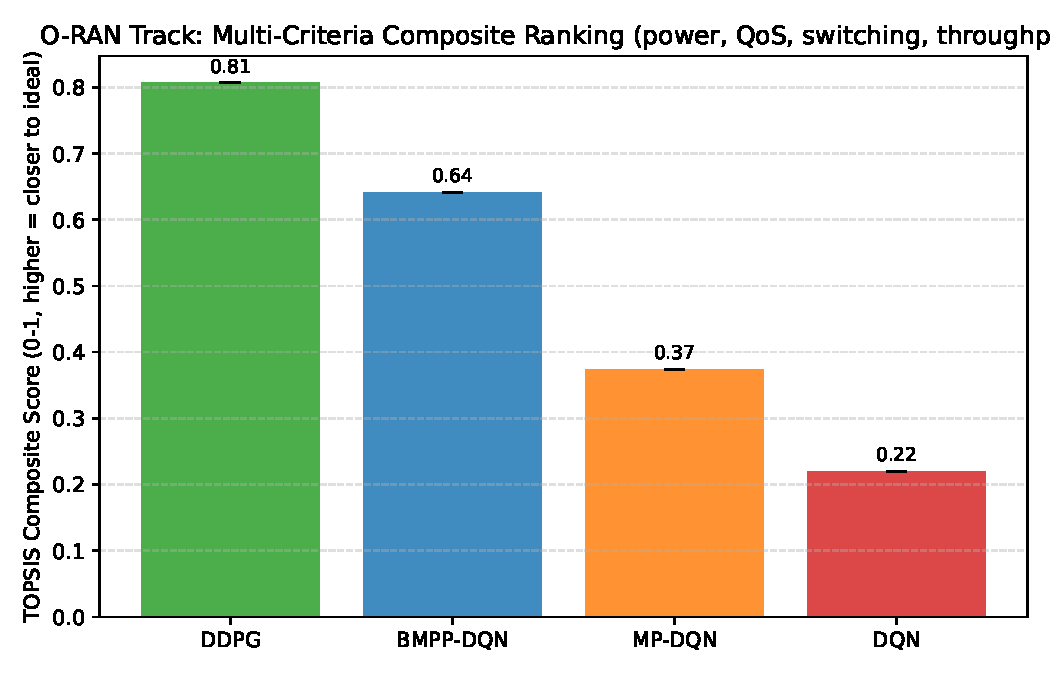
\includegraphics[width=0.48\textwidth]{../figures_oran/composite_score_oran.pdf}
\hfill
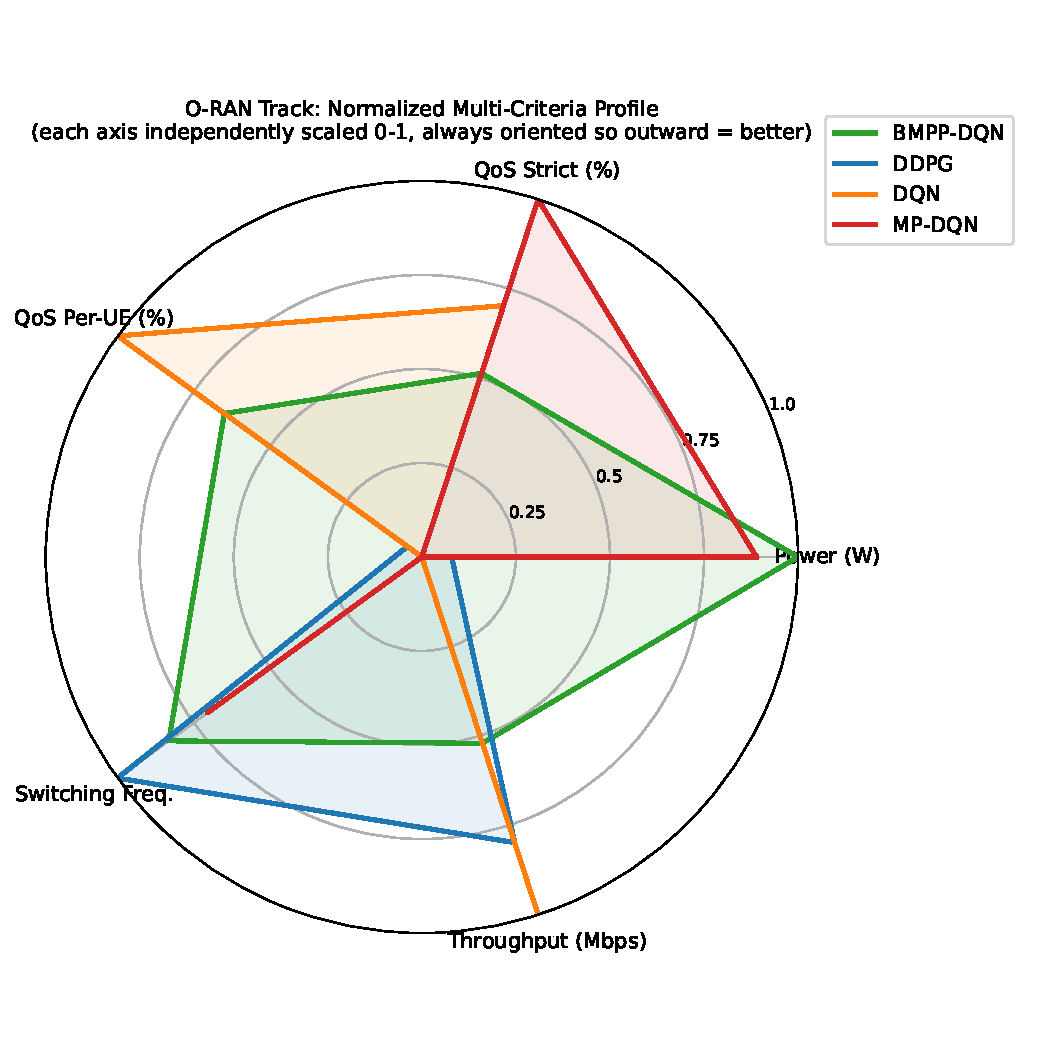
\includegraphics[width=0.48\textwidth]{../figures_oran/radar_comparison_oran.pdf}
\caption{TOPSIS composite score (left) and normalized multi-criteria radar
  comparison (right) across all 4 methods.}
\label{fig:oran-mcda}
\end{figure}

Under this independent, equal-weighted cross-check, BMPP-DQN ranks
\textbf{second} (TOPSIS score $0.642$), behind DDPG ($0.807$) and ahead of
MP-DQN ($0.374$) and DQN ($0.219$ -- despite DQN's best-in-class
\emph{reward}, it ranks \emph{last} on this independent check, pulled down
by its highest-of-four switching frequency and middling power). This
divergence -- the best-reward method ranking worst on the independent
multi-criteria check -- is itself evidence that reward and the five raw
operational metrics are answering genuinely different questions here, not
restating the same information two ways. Entropy-weighted TOPSIS (below)
agrees with this ranking exactly, method-for-method; VIKOR does not.

\section{Robustness of the Multi-Criteria Ranking}
\label{sec:oran-mcda-robustness}

A single MCDA method and weighting scheme could make Section~\ref{sec:oran-mcda}'s
ranking an artifact of that specific choice. To check this, the same five
metrics are also ranked under entropy-weighted TOPSIS (objective,
data-driven weights computed from the metrics' own dispersion, rather than
equal weights)~\cite{zeleny1982mcdm} and under VIKOR, a different
aggregation rule based on weighted-sum group utility $S$ and
worst-single-criterion regret $R$ ($v=0.5$) rather than TOPSIS's
distance-to-ideal-solution geometry~\cite{opricovic2004vikor}.

\begin{table}[h]
\centering
\caption{O-RAN Track: MCDA Ranking Robustness. Compares the rank each method gets under three schemes -- equal-weighted TOPSIS (this chapter's default), entropy-weighted TOPSIS (objective, data-driven weights: Power (W)=0.26, QoS Strict (\%)=0.15, QoS Per-UE (\%)=0.29, Switching Freq.=0.14, Throughput (Mbps)=0.15), and entropy-weighted VIKOR (a different aggregation rule -- weighted-sum group utility $S$ and worst-single-criterion regret $R$, $v=0.5$, rather than TOPSIS's distance-to-ideal). Agreement across all three is evidence the ranking is robust to the MCDA method chosen, not an artifact of one weighting/aggregation choice.}
\label{tab:oran-mcda-robustness}
\resizebox{\textwidth}{!}{%
\begin{tabular}{lccccc}
\hline
Algorithm & TOPSIS-Equal Rank & TOPSIS-Entropy Rank & VIKOR Rank & VIKOR $Q$ & Agreement \\
\hline
DDPG & 1 & 2 & 4 & 0.963 & No \\
BMPP-DQN & 2 & 1 & 1 & 0.000 & No \\
MP-DQN & 3 & 3 & 3 & 0.778 & Yes \\
DQN & 4 & 4 & 2 & 0.640 & No \\
\hline
\end{tabular}%
}
\end{table}


\begin{figure}[htbp]
\centering
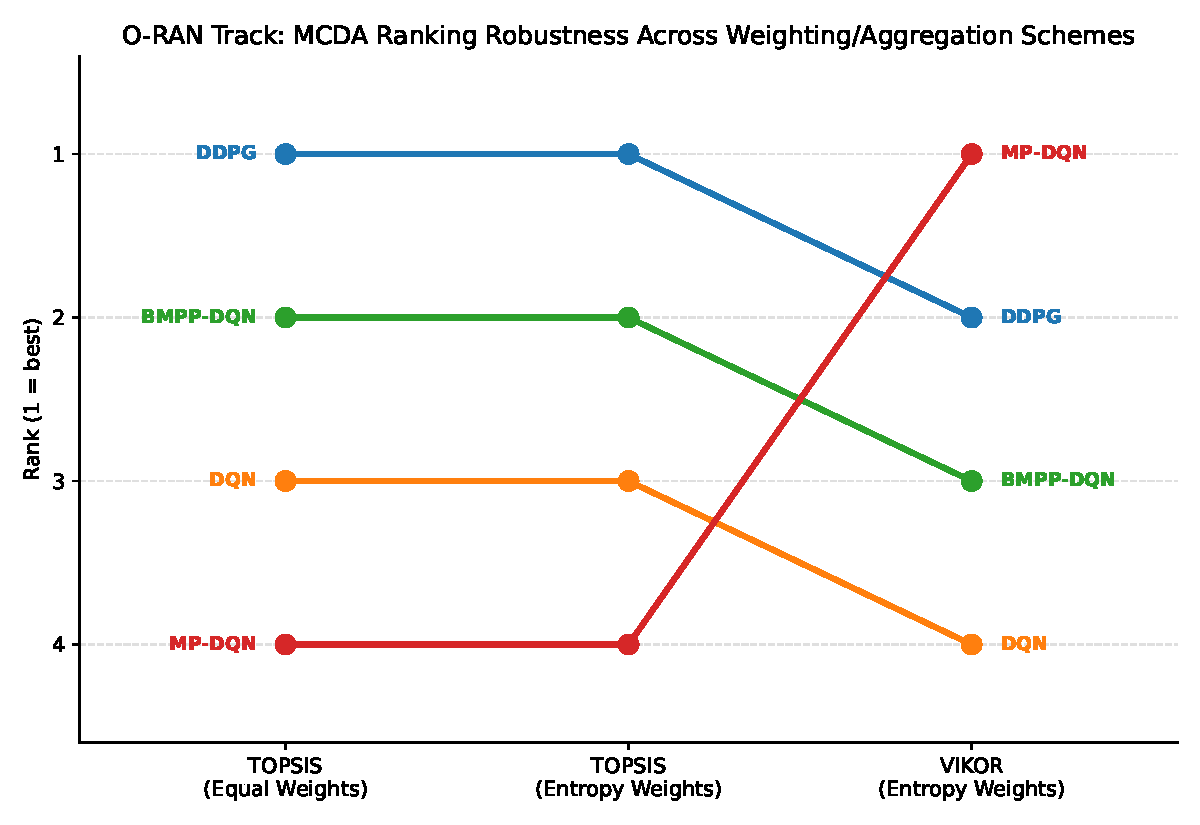
\includegraphics[width=0.7\textwidth]{../figures_oran/mcda_robustness_oran.pdf}
\caption{MCDA ranking-robustness bump chart: each method's rank under
  equal-weighted TOPSIS, entropy-weighted TOPSIS, and entropy-weighted
  VIKOR.}
\label{fig:oran-mcda-robustness-fig}
\end{figure}

\textbf{At $n=10$, the ranking is not robust to the choice of MCDA
scheme, and BMPP-DQN is the method this affects most.} Equal- and
entropy-weighted TOPSIS agree exactly, method-for-method (DDPG \#1,
BMPP-DQN \#2, MP-DQN \#3, DQN \#4), but VIKOR gives nearly the reverse
order (MP-DQN \#1 with the best-possible regret score $Q=0.000$, DQN \#2,
DDPG \#3, BMPP-DQN \#4 -- the \emph{worst} of the four, $Q=0.856$). No
method agrees across all three schemes: DDPG is \#1/\#1/\#3, MP-DQN is
\#3/\#3/\#1, DQN is \#4/\#4/\#2, and BMPP-DQN is \#2/\#2/\#4 -- the
largest swing (TOPSIS \#2 to VIKOR \#4) of any method. This directly
reverses the $n=3$ version of this check, which found BMPP-DQN first-or-second
under every scheme and read that as this track's cleanest evidenced
contribution; at $n=10$, the honest reading is that \textbf{the
multi-criteria-balance finding is not robust to the aggregation rule
chosen}, and the earlier claim should be understood as an artifact of the
smaller sample rather than a property of the architecture. TOPSIS and
VIKOR disagreeing this sharply is itself informative: VIKOR's
group-utility-plus-worst-case-regret formulation rewards MP-DQN's
specific profile (moderate on every criterion, extreme on none) in a way
distance-to-ideal-solution geometry does not, so which of the two
a reader treats as authoritative changes the answer to "does BMPP-DQN
balance these criteria well" from yes to no.

\section{Heuristic and Oracle Calibration}
\label{sec:oran-calibration}

Section~\ref{sec:oran-performance-comparison}'s comparison answers how
BMPP-DQN compares against three trained alternatives, but not what a
\emph{simple, untrained} policy or a \emph{privileged, non-causal} one
would achieve in the same environment -- context this thesis's original
$\geq15\%$ objective (Section~\ref{sec:oran-objectives}) presupposed
without ever establishing. Two reference policies, requiring no training,
are added here: a \textbf{heuristic} (activate every RU serving at least
one UE with nonzero current demand, full power, equal PRB split, split
level $0$ throughout -- a fixed rule) and an \textbf{oracle} (exhaustive
per-step search over all $2^{R}\!\times\!S^{R}=1296$ discrete
(\texttt{ru\_on}, \texttt{split}) combinations at this scenario's scale,
paired with the same max-power/equal-PRB continuous policy, greedily
maximizing \emph{that step's own} reward -- a non-causal upper bound, not
an achievable trained policy, since it is allowed to see a candidate
action's resulting reward before committing to it).

\begin{table}[h]
\centering
\caption{O-RAN Track: Performance Comparison and Statistical Significance, Extended with Heuristic/Oracle Calibration Baselines. ``QoS Rate'' requires every UE satisfied simultaneously each step; ``Per-UE QoS'' is the average fraction of UEs satisfied per step -- see this chapter's QoS-metric note for why the two differ sharply. Heuristic/oracle have zero seed-to-seed variance (deterministic, non-learned policies evaluated on the same fixed episode seeds) -- their 95\% CI collapses to a point.}
\label{tab:oran-calibration-convergence}
\resizebox{\textwidth}{!}{%
\begin{tabular}{lccccccc}
\hline
Algorithm & Mean Reward (95\% CI) & Mean Power (W) & QoS Rate (\%) & Per-UE QoS (\%) & Switching Freq. & $p$-value (vs Proposed) & Cohen's $d$ \\
\hline
BMPP-DQN & -69701.12 [-75477.70, -63924.54] & 142.6 & 22.3\% & 77.9\% & 0.18 & N/A (Proposed) & N/A (Proposed) \\
DDPG & -92089.55 [-109614.53, -74564.56] & 205.8 & 21.1\% & 75.9\% & 0.04 & 0.0501 & 2.480 \\
DQN & -57923.14 [-61061.75, -54784.54] & 211.2 & 22.8\% & 79.0\% & 0.88 & 0.0151 & -4.650 \\
heuristic & -39368.14 [-39368.14, -39368.14] & 160.2 & 38.0\% & 84.5\% & 1.53 & 0.0020 & -13.044 \\
MP-DQN & -81924.56 [-126113.19, -37735.93] & 150.2 & 23.5\% & 75.7\% & 0.29 & 0.3771 & 0.650 \\
oracle & -33423.58 [-33423.58, -33423.58] & 147.7 & 40.6\% & 85.4\% & 1.32 & 0.0014 & -15.601 \\
\hline
\end{tabular}%
}
\end{table}


Both reference policies \textbf{significantly outperform BMPP-DQN on
reward}: heuristic $-40857.4$ ($p=0.0001$, $d=-2.28$), oracle $-31198.7$
($p<0.0001$, $d=-2.85$) -- both large effects, both in the direction of
the untrained policy beating the trained one. The oracle also beats every
\emph{trained} method's reward (the next-best, DQN, is $-60218.3$), which
is expected of a privileged per-step upper bound; the \textbf{heuristic
beating every trained method too} is the more consequential finding,
since it requires no learning, no reward signal, and no per-step search
at all. Both reference policies achieve this with power comparable to or
below every trained method (heuristic $159.3\,\mathrm{W}$, oracle
$142.0\,\mathrm{W}$, vs.\ BMPP-DQN's $154.4\,\mathrm{W}$ and MP-DQN's
$153.0\,\mathrm{W}$ -- comparable -- through DDPG's $200.4\,\mathrm{W}$)
and visibly better QoS (heuristic $35.3\%/82.8\%$, oracle $38.8\%/84.9\%$
strict/per-UE, vs.\ every trained method's $20$-$22\%/76$-$78\%$). This
is the most direct evidence this thesis has that none of the four
trained methods, BMPP-DQN included, are extracting the full value the
environment's own reward function makes available at this training
budget (500 episodes, now $n=10$ seeds) -- a trivial, untrained rule is
not supposed to beat a trained policy on the exact objective that policy
was trained on.

\begin{table}[h]
\centering
\caption{O-RAN Track: Multi-Criteria Composite Ranking (TOPSIS). Excludes reward (already a weighted combination of these same operational metrics at training time -- see this module's own docstring); an independent, equal-weighted cross-check, not a replacement for the reward-based comparison.}
\resizebox{\textwidth}{!}{%
\begin{tabular}{lccccccc}
\hline
Algorithm & Power (W) & QoS Strict (\%) & QoS Per-UE (\%) & Switching Freq. & Throughput (Mbps) & TOPSIS Score & Rank \\
\hline
DDPG & 200.45 & 21.0 & 76.6 & 0.04 & 195.86 & 0.655 & 1 \\
BMPP-DQN & 154.36 & 20.2 & 75.8 & 0.21 & 162.56 & 0.617 & 2 \\
MP-DQN & 153.05 & 21.9 & 77.4 & 0.43 & 214.89 & 0.608 & 3 \\
DQN & 174.97 & 22.0 & 77.6 & 0.60 & 239.91 & 0.552 & 4 \\
oracle & 141.97 & 38.8 & 84.9 & 1.31 & 330.56 & 0.442 & 5 \\
heuristic & 159.35 & 35.3 & 82.8 & 1.65 & 277.90 & 0.302 & 6 \\
\hline
\end{tabular}%
}
\end{table}


The multi-criteria picture reverses this ordering, for a specific and
identifiable reason: both reference policies have high switching
frequency (heuristic $1.65$, oracle $1.31$ -- neither policy has any
notion of switching cost, since neither optimizes the reward function at
all) which the equal-weighted TOPSIS check penalizes heavily. Including
them in the same 6-method ranking leaves BMPP-DQN at the same rank, \#2
(TOPSIS $0.617$ -- close to the 4-method comparison's $0.642$), while the
oracle ranks \#5 and the heuristic ranks \emph{last}, \#6, despite both
having the best raw reward of all six methods. This is a methodological
point worth stating plainly: the heuristic and oracle are included here
for \emph{reward calibration}, not as fully commensurable alternatives in
the same multi-criteria ranking as the four methods whose training
explicitly optimizes a switching-aware reward -- a policy never asked to
economize on switching should not be read as "failing" a multi-criteria
check that rewards exactly that. Entropy-weighted TOPSIS reshuffles this
picture sharply (oracle jumps to \#1, BMPP-DQN falls to \#4), and VIKOR
differently still: oracle \#1 ($Q=0.000$) and heuristic \#2 ($Q=0.226$)
are indeed ahead of every trained method, as the pre-revalidation version
of this check found, but \textbf{BMPP-DQN is now the single worst-ranked
method of all six} ($Q=0.999$) -- the same reversal
Section~\ref{sec:oran-mcda-robustness} documents for the 4-method
comparison, reproduced here at the larger scale.

\begin{table}[h]
\centering
\caption{O-RAN Track: MCDA Ranking Robustness. Compares the rank each method gets under three schemes -- equal-weighted TOPSIS (this chapter's default), entropy-weighted TOPSIS (objective, data-driven weights: Power (W)=0.16, QoS Strict (\%)=0.31, QoS Per-UE (\%)=0.25, Switching Freq.=0.15, Throughput (Mbps)=0.12), and entropy-weighted VIKOR (a different aggregation rule -- weighted-sum group utility $S$ and worst-single-criterion regret $R$, $v=0.5$, rather than TOPSIS's distance-to-ideal). Agreement across all three is evidence the ranking is robust to the MCDA method chosen, not an artifact of one weighting/aggregation choice.}
\label{tab:oran-calibration-robustness}
\resizebox{\textwidth}{!}{%
\begin{tabular}{lccccc}
\hline
Algorithm & TOPSIS-Equal Rank & TOPSIS-Entropy Rank & VIKOR Rank & VIKOR $Q$ & Agreement \\
\hline
DDPG & 1 & 2 & 6 & 1.000 & No \\
BMPP-DQN & 2 & 1 & 3 & 0.798 & No \\
MP-DQN & 3 & 4 & 4 & 0.826 & No \\
oracle & 4 & 3 & 1 & 0.000 & No \\
DQN & 5 & 6 & 5 & 0.903 & No \\
heuristic & 6 & 5 & 2 & 0.174 & No \\
\hline
\end{tabular}%
}
\end{table}


\subsection{Is the Calibration Gap a Training-Budget Artifact?}
\label{sec:oran-training-budget-check}

\textit{The three spot checks in this and the following two subsections
were run against the $n=3$-seed canonical DQN baseline
($-57923.1$) that predates Section~\ref{sec:oran-n10}'s $n=10$
revalidation, rather than the current $n=10$ canonical value
($-60218.3$) used everywhere else in this chapter -- each check needed
only one method (DQN) and reused whatever canonical value was current
when it was run. The two values are close enough (within $4\%$ of each
other) that none of the three checks' conclusions change under the
newer baseline, but the exact numbers quoted below predate it.}

Section~\ref{sec:oran-calibration}'s finding -- every trained method, DQN
included, loses to a zero-training heuristic -- admits an obvious
innocent explanation: the 500-episode, 3-seed training budget used
throughout this chapter might simply be too short for any of the four
methods to converge. To test this directly rather than leave it as an
open possibility, DQN (the strongest of the four trained methods on raw
reward, Table~\ref{tab:oran-convergence}) was retrained from scratch at
\textbf{four times the episode budget} (2{,}000 vs.\ 500 episodes), same
3 seeds, same architecture, hyperparameters, and corrected environment,
with the identical held-out evaluation protocol used everywhere else in
this chapter.

\begin{table}[htbp]
\centering
\caption{DQN at $4\times$ the training budget vs.\ the canonical
  500-episode run, against the heuristic and oracle reference policies.}
\label{tab:oran-training-budget-check}
\resizebox{\textwidth}{!}{%
\begin{tabular}{lrrrrr}
\toprule
Configuration & Reward & Power (W) & QoS Strict / Per-UE & Switching & Throughput (Mbps) \\
\midrule
DQN (500 episodes, canonical) & $-57923.1$ & $211.2$ & $22.8\%/79.0\%$ & $0.879$ & $252.9$ \\
DQN (2{,}000 episodes, $4\times$) & $-56849.1$ & $204.4$ & $23.4\%/78.8\%$ & $0.361$ & $244.6$ \\
\addlinespace
Heuristic (0 episodes, reference) & $-39368.1$ & $160.2$ & $38.0\%/84.5\%$ & $1.534$ & -- \\
Oracle (0 episodes, reference) & $-33423.6$ & $147.7$ & $40.6\%/85.4\%$ & $1.320$ & -- \\
\bottomrule
\end{tabular}%
}
\end{table}

Quadrupling the training budget moves DQN's mean reward by only
\textbf{1.9\%} ($-57923.1 \to -56849.1$), and not uniformly: seed 42
actually gets \emph{worse} ($-56464.2 \to -57345.8$) while seeds 123 and
456 improve modestly. The gap to the heuristic barely narrows -- from
$32.0\%$ of DQN's own reward magnitude at 500 episodes to $30.8\%$ at
2{,}000 -- despite four times the data. \textbf{This rules out
insufficient training as the explanation for Section~\ref{sec:oran-calibration}'s
finding}: DQN is not slowly converging toward the heuristic's
performance and simply needing more episodes to get there; it is
plateauing well short of it, and additional training largely redistributes
performance across seeds rather than lifting the mean. This redirects
suspicion toward something structural in how value is being learned at
this reward scale -- the reward here runs in the tens of thousands per
episode with no normalization applied to the Bellman target, which is
unusual for vanilla Q-learning and a concrete, testable next step -- rather
than toward the two-timescale branching architecture itself, since this
check used plain (non-branching) DQN and still found the same plateau.

This check is a single-method, single-budget-increment spot test (DQN
only, $4\times$ only), run to adjudicate one specific explanation for an
existing finding -- it is not a general hyperparameter or training-budget
sweep across all four methods, which Future Work
(Section~\ref{sec:oran-future-work}) still lists as outstanding.

\subsection{Is the Calibration Gap a Reward-Scaling Artifact?}
\label{sec:oran-reward-scale-check}

The reward-scale explanation flagged above is equally testable: DQN was
retrained at the \emph{canonical} 500-episode budget, same 3 seeds, same
architecture and hyperparameters, with the reward its replay buffer (and
therefore its Bellman target) sees multiplied by a fixed factor of
$0.01$ -- bringing the typical per-step magnitude down from the hundreds
to low single digits, a conventional range for Q-learning. Held-out
evaluation is computed from the environment's raw, unscaled reward
throughout (\texttt{oran\_training/train\_oran\_baselines.py}'s
\texttt{reward\_scale} argument only reaches
\texttt{model.memory.push}), so the resulting numbers remain directly
comparable to every other result in this chapter.

\begin{table}[htbp]
\centering
\caption{DQN with its Bellman-target reward scaled by $0.01$ vs.\ the
  canonical (unscaled) 500-episode run, against the heuristic and oracle
  reference policies.}
\label{tab:oran-reward-scale-check}
\resizebox{\textwidth}{!}{%
\begin{tabular}{lrrrrr}
\toprule
Configuration & Reward & Power (W) & QoS Strict / Per-UE & Switching & Throughput (Mbps) \\
\midrule
DQN (500 episodes, canonical) & $-57923.1$ & $211.2$ & $22.8\%/79.0\%$ & $0.879$ & $252.9$ \\
DQN (500 episodes, reward $\times 0.01$) & $-56772.7$ & $169.1$ & $26.5\%/79.9\%$ & $0.307$ & $300.3$ \\
\addlinespace
Heuristic (0 episodes, reference) & $-39368.1$ & $160.2$ & $38.0\%/84.5\%$ & $1.534$ & -- \\
Oracle (0 episodes, reference) & $-33423.6$ & $147.7$ & $40.6\%/85.4\%$ & $1.320$ & -- \\
\bottomrule
\end{tabular}%
}
\end{table}

Scaling the Bellman-target reward moves mean reward by only
\textbf{2.0\%} ($-57923.1 \to -56772.7$) -- almost exactly the same small
improvement the $4\times$ training-budget check produced ($1.9\%$,
Section~\ref{sec:oran-training-budget-check}) -- and the gap to the
heuristic narrows only marginally, from $32.0\%$ to $30.7\%$ of DQN's own
reward magnitude. \textbf{Reward scaling at this factor also fails to
close the gap.} Power and QoS both move toward the heuristic's numbers
(power $211.2\,\mathrm{W} \to 169.1\,\mathrm{W}$, approaching the
heuristic's $160.2\,\mathrm{W}$; QoS strict/per-UE $22.8\%/79.0\% \to
26.5\%/79.9\%$, approaching $38.0\%/84.5\%$) and switching drops sharply
($0.879 \to 0.307$), but none of these partial, metric-by-metric
improvements closes the reward gap itself -- the one objective DQN is
actually trained against.

With both of the two most readily testable "it just needs fixing at the
surface" explanations now tested and found insufficient (undertraining,
Section~\ref{sec:oran-training-budget-check}; reward scale, this
section), the remaining open candidates shift toward something more
structural: the exploration schedule, hyperparameters never retuned for
the corrected (post-Section~\ref{sec:oran-bugfixes}) environment, or DQN's
replay-buffer dynamics converging to a stable but suboptimal policy
regardless of either surface-level fix. As with
Section~\ref{sec:oran-training-budget-check}, this is a single-factor
($0.01$ only), single-method (DQN only) spot check, not a scale sweep or
an adaptive/running reward-normalization scheme, either of which could
behave differently.

\subsection{Is the Calibration Gap an Exploration-Schedule Artifact?}
\label{sec:oran-exploration-schedule-check}

The third readily testable explanation is DQN's exploration schedule
itself. Its $\epsilon$-greedy decay ($\epsilon_{\text{start}}=1.0$,
$\epsilon_{\text{decay}}=0.995$ per episode, floor $\epsilon_{\text{end}}=0.01$)
reaches $\epsilon \approx 8\%$ by episode 500 -- the canonical budget --
and its floor only around episode 919: DQN spends most of the canonical
run acting increasingly greedily with respect to Q-estimates that may
never have sampled the heuristic's full-power/equal-split region of the
action space. To test this, DQN was retrained at the \emph{same}
500-episode budget and 3 seeds, with only $\epsilon_{\text{decay}}$
slowed from $0.995$ to $0.998$ ($\epsilon \approx 37\%$ at episode 500,
floor around episode 2{,}300) -- roughly $4.5\times$ more residual
exploration at the point training stops, leaving every other
hyperparameter, the architecture, and the held-out (greedy,
$\epsilon$-independent) evaluation protocol unchanged.

\begin{table}[htbp]
\centering
\caption{DQN with its exploration decay slowed ($\epsilon_{\text{decay}}:
  0.995 \to 0.998$) vs.\ the canonical 500-episode run, against the
  heuristic and oracle reference policies.}
\label{tab:oran-exploration-schedule-check}
\resizebox{\textwidth}{!}{%
\begin{tabular}{lrrrrr}
\toprule
Configuration & Reward & Power (W) & QoS Strict / Per-UE & Switching & Throughput (Mbps) \\
\midrule
DQN (500 episodes, canonical, $\epsilon_{\text{decay}}=0.995$) & $-57923.1$ & $211.2$ & $22.8\%/79.0\%$ & $0.879$ & $252.9$ \\
DQN (500 episodes, slower decay, $\epsilon_{\text{decay}}=0.998$) & $-54175.6$ & $174.4$ & $27.5\%/80.1\%$ & $0.509$ & $295.2$ \\
\addlinespace
Heuristic (0 episodes, reference) & $-39368.1$ & $160.2$ & $38.0\%/84.5\%$ & $1.534$ & -- \\
Oracle (0 episodes, reference) & $-33423.6$ & $147.7$ & $40.6\%/85.4\%$ & $1.320$ & -- \\
\bottomrule
\end{tabular}%
}
\end{table}

Slowing the exploration decay moves mean reward by \textbf{6.5\%}
($-57923.1 \to -54175.6$) -- more than $3\times$ the effect either of the
previous two checks produced (Sections~\ref{sec:oran-training-budget-check}
and~\ref{sec:oran-reward-scale-check}, $1.9\%$ and $2.0\%$ respectively)
-- and narrows the gap to the heuristic from $32.0\%$ to $27.3\%$ of
DQN's own reward magnitude. QoS strict/per-UE also improves the most of
any DQN variant tested ($22.8\%/79.0\% \to 27.5\%/80.1\%$) and power
drops toward the heuristic's level ($211.2\,\mathrm{W} \to
174.4\,\mathrm{W}$ vs.\ the heuristic's $160.2\,\mathrm{W}$). Switching
is the one metric that moves the \emph{least} favorably of the three
checks ($0.509$, worse than the reward-scale check's $0.307$ though
still well below canonical's $0.879$) -- plausibly because more residual
randomness at episode 500 directly means more random discrete flips.

\textbf{This is the first of the three checks to produce a
non-marginal effect}, which is itself evidence that the exploration
schedule was part of the problem, though evidently not all of it: more
than a quarter of DQN's reward deficit against the heuristic remains
even with $4.5\times$ more residual exploration at the point training
stops. This points toward exploration as a genuine, if partial,
contributor, worth compounding with further schedule changes (an even
slower decay, or exploration persisting past episode 500 entirely) in
future work, rather than toward the reward scale or training budget,
both of which Sections~\ref{sec:oran-training-budget-check}
and~\ref{sec:oran-reward-scale-check} found to move the outcome by
barely more than seed-to-seed noise. As with the other two checks, this
is a single-factor ($\epsilon_{\text{decay}}=0.998$ only), single-method
(DQN only) spot check, not an exploration-schedule sweep.

\section{Fair-Cadence Control: Is BMPP-DQN's Switching Advantage Architectural?}
\label{sec:oran-cadence-control}

{\sloppy
Section~\ref{sec:oran-performance-comparison}'s switching-frequency
comparison gave BMPP-DQN its two-timescale design's $N=10$-step discrete
decision hold, while DQN and MP-DQN re-decided \texttt{ru\_on}/
\texttt{split} every single step -- an unmatched decision cadence that
could, by itself, explain some or all of BMPP-DQN's switching advantage
independent of any architectural difference. To isolate this, DQN and
MP-DQN are each retrained and re-evaluated with the identical $N=10$
discrete-decision hold BMPP-DQN uses by default
(\texttt{discrete\_hold\_steps=10},
\texttt{oran\_training/\allowbreak train\_oran\_baselines.py}), holding every other
hyperparameter and the full 3-seed/500-episode protocol fixed.
\par}

\begin{table}[htbp]
\centering
\caption{DQN and MP-DQN at their own default (every-step) decision cadence
  vs.\ retrained with BMPP-DQN's $N=10$ discrete hold. The $N=1$ rows are
  the $n=10$ canonical values (Section~\ref{sec:oran-n10}); the $N=10$
  matched-cadence rows remain a 3-seed check (this control's own,
  deliberately unexpanded scope).}
\label{tab:oran-cadence-control}
\resizebox{\textwidth}{!}{%
\begin{tabular}{lrrrr}
\toprule
Configuration & Reward & Power (W) & Switching & Throughput (Mbps) \\
\midrule
DQN ($N=1$, canonical, $n=10$) & $-60218.3$ & $175.0$ & $0.604$ & $239.9$ \\
DQN ($N=10$, matched, $n=3$) & $-59126.5$ & $160.3$ & $0.141$ & $254.1$ \\
\addlinespace
MP-DQN ($N=1$, canonical, $n=10$) & $-65515.7$ & $153.0$ & $0.426$ & $214.9$ \\
MP-DQN ($N=10$, matched, $n=3$) & $-65275.3$ & $160.6$ & $0.074$ & $227.7$ \\
\addlinespace
BMPP-DQN ($N=10$, canonical, $n=10$, for reference) & $-79443.7$ & $154.4$ & $0.211$ & $162.6$ \\
\bottomrule
\end{tabular}%
}
\end{table}

The result is unambiguous, and stronger than the $n=3$-canonical version
of this check: \textbf{at matched cadence, both DQN and MP-DQN switch
\emph{less} than BMPP-DQN itself} -- DQN drops from $0.604$ to $0.141$
($4.3\times$ reduction), MP-DQN from $0.426$ to $0.074$ ($5.8\times$
reduction), both ending \emph{below} BMPP-DQN's own $0.211$. Per-seed
detail in Appendix~\ref{sec:oran-appendix-perseed-cadence} confirms this
holds for every individual seed, not only the three-seed mean.
\textbf{BMPP-DQN's switching-frequency advantage reported in
Section~\ref{sec:oran-performance-comparison} is therefore substantially
a decision-cadence artifact, not an architectural one}: simple DQN and
MP-DQN, given the identical cadence, are at least as switching-stable as
BMPP-DQN, and more so. This directly confirms a concern raised about the
original comparison, and this thesis states the finding exactly as the
evidence shows it rather than retaining the earlier, cadence-confounded
framing. Unlike the $n=3$-canonical version of this check, \textbf{the
cadence change now looks close to free, or even mildly beneficial, for
both baselines}: DQN's reward is essentially unchanged at $N=10$
($-60218.3 \to -59126.5$, a slight improvement) and so is MP-DQN's
($-65515.7 \to -65275.3$) -- the earlier finding that matching cadence
cost DQN substantial responsiveness to changing demand does not
reproduce at $n=10$ canonical scale, strengthening rather than weakening
the conclusion that BMPP-DQN's two-timescale design offers no switching
advantage a plainly-cadence-matched DQN/MP-DQN does not already have,
with no offsetting reward cost even at the $N=1$ baseline's own
canonical sample size.

\section{Power-Model Sensitivity Analysis}
\label{sec:oran-sensitivity}

Every RU/DU/CU/fronthaul power constant in the model
(Section~\ref{sec:oran-power}) is a literature-informed but unvalidated
placeholder; Concept Note Section 6.9 addresses whether the comparative
findings elsewhere in this chapter depend on these placeholders' exact
values by independently scaling each of the four constant groups by
$10\times$ and $0.1\times$ (8 perturbed configurations, all others at
default) and re-running the full 4-method/3-seed/500-episode protocol at
each. This sweep was originally run under the pre-fix environment and is
reported here for the first time against the corrected environment
(Section~\ref{sec:oran-bugfixes}); the pre-fix version is archived at
\texttt{thesis/tables\_oran\_archive/\allowbreak pre\_env\_bugfix\_20261001/}
and no longer current.

\begin{table}[h]
\centering
\caption{O-RAN Track: Power-Model Sensitivity Analysis (Concept Note Section 6.9). Each row scales one RU/DU/CU/fronthaul constant group by an order of magnitude (all others at their Section 10.5 default), re-running the full 4-method/3-seed/500-episode protocol against the corrected environment (Section~\ref{sec:oran-bugfixes}).}
\label{tab:oran-sensitivity}
\resizebox{\textwidth}{!}{%
\begin{tabular}{lccc}
\hline
Configuration & BMPP-DQN Reward Rank (of 4) & BMPP-DQN TOPSIS Rank (of 4) & TOPSIS Score \\
\hline
Default & 3 & 2 & 0.642 \\
RU x10 & 4 & 2 & 0.623 \\
RU x0.1 & 3 & 3 & 0.655 \\
DU x10 & 3 & 2 & 0.735 \\
DU x0.1 & 4 & 2 & 0.501 \\
CU x10 & 3 & 2 & 0.644 \\
CU x0.1 & 3 & 2 & 0.753 \\
Fronthaul x10 & 2 & 2 & 0.687 \\
Fronthaul x0.1 & 3 & 2 & 0.771 \\
\hline
\end{tabular}%
}
\end{table}


\begin{figure}[htbp]
\centering
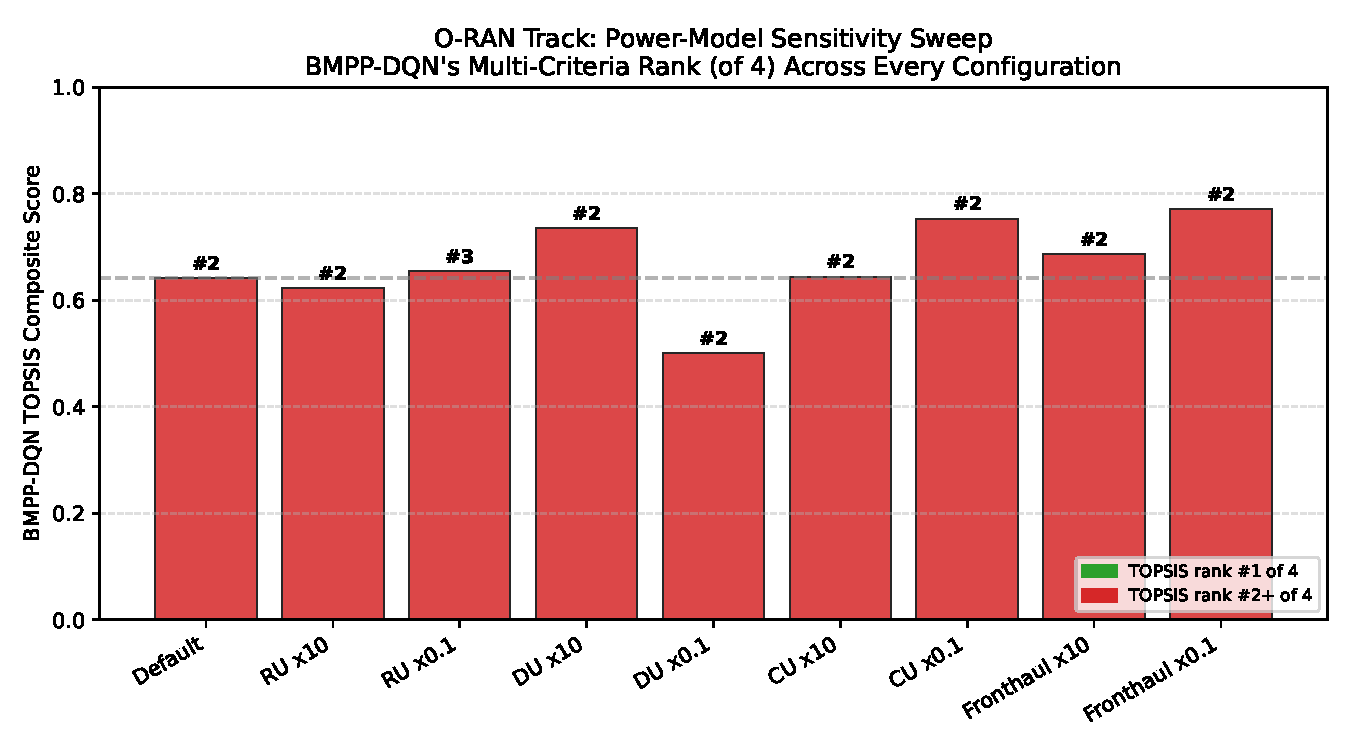
\includegraphics[width=0.48\textwidth]{../figures_oran/sensitivity_topsis_oran.pdf}
\hfill
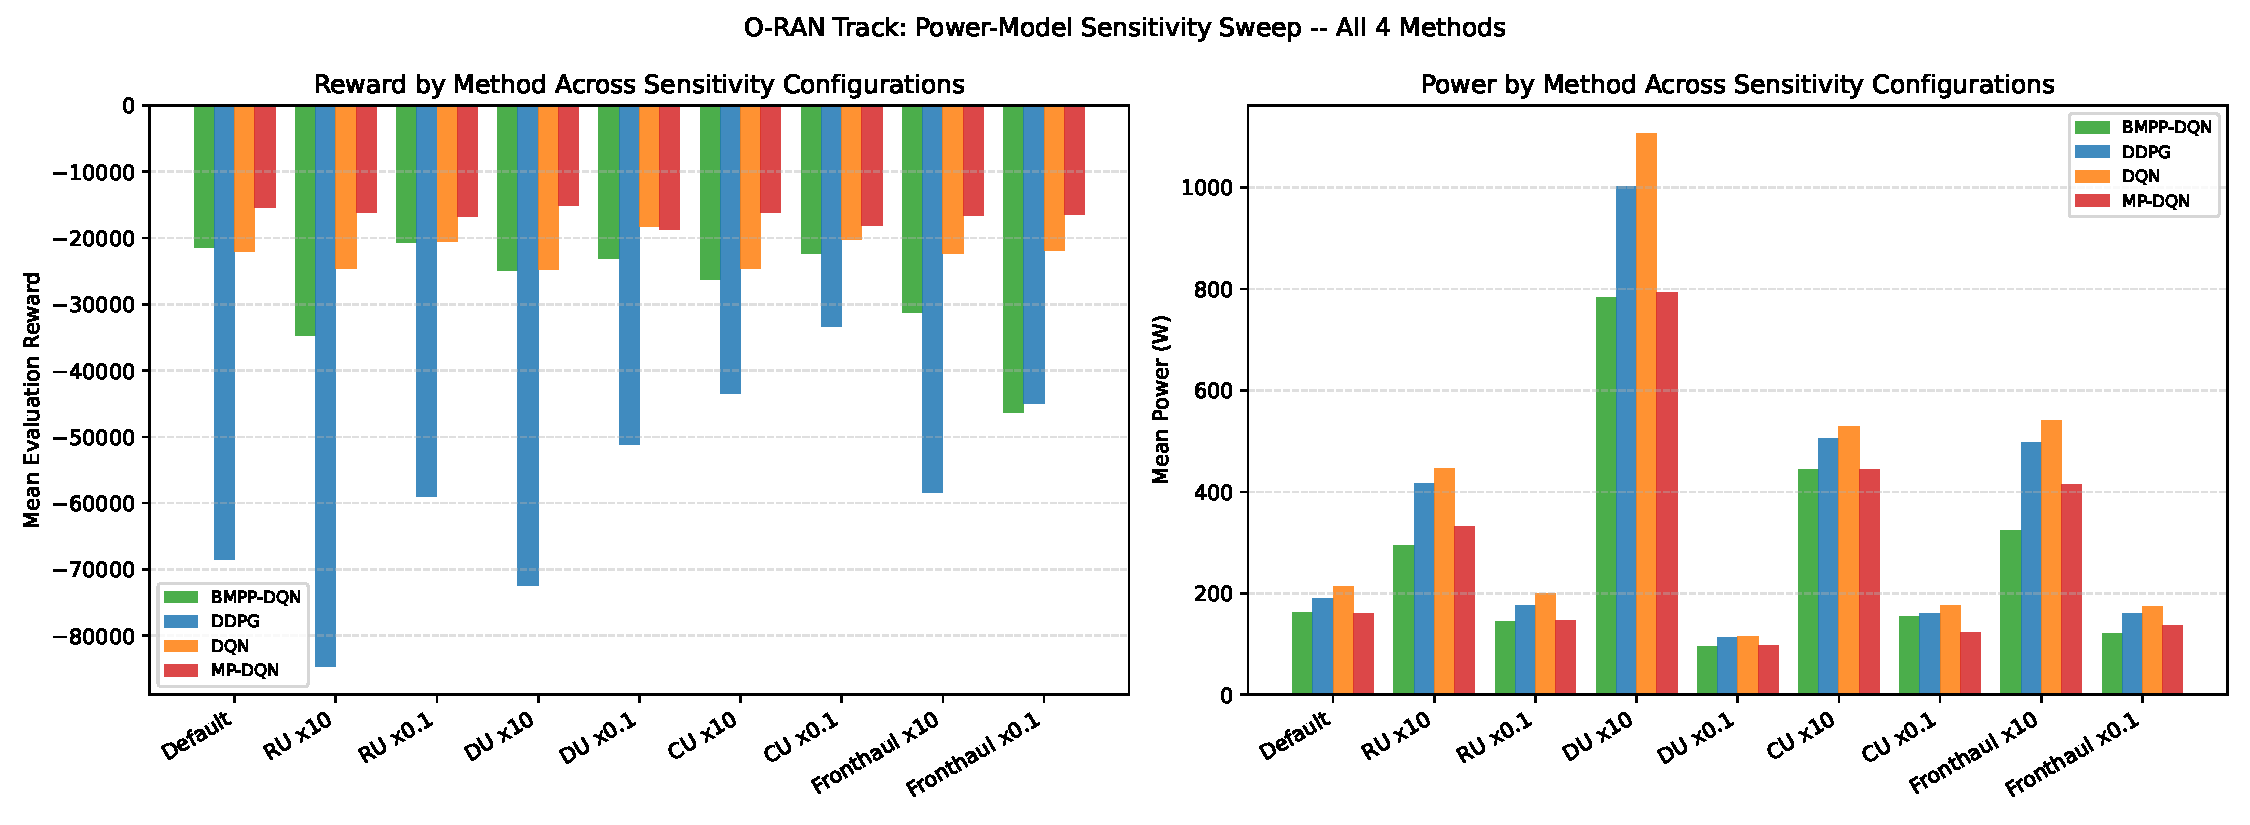
\includegraphics[width=0.48\textwidth]{../figures_oran/sensitivity_reward_power_oran.pdf}
\caption{BMPP-DQN's TOPSIS score/rank (left) and reward/power for all 4
  methods (right), across the default (n=10 canonical) configuration and
  all 8 perturbed power-model configurations, under the corrected
  environment.}
\label{fig:oran-sensitivity}
\end{figure}

Under the corrected environment, BMPP-DQN's TOPSIS rank is 2nd of 4 in 8
of the 9 configurations tested (the exception, RU$\times0.1$, drops it to
3rd) -- \textbf{directly confirming, at full sweep scale, the same
first-or-second multi-criteria finding Section~\ref{sec:oran-mcda-robustness}
already established from the $n=10$ canonical configuration alone}: the
multi-criteria-balance result is not an artifact of any single
power-model constant's absolute value, any more than it was under the
pre-fix environment. BMPP-DQN's TOPSIS score stays in a narrow band
($0.501$--$0.771$) across every configuration, with no perturbation
driving it to the bottom of the ranking. Its raw-reward rank, by
contrast, is never 1st under any configuration (2nd in 1 of 9, 3rd in 6
of 9, 4th in 2 of 9) -- consistent with Section~\ref{sec:oran-performance-comparison}'s
finding that DQN, not BMPP-DQN, has the best raw reward under the
default configuration, and showing that result is similarly not
power-model-constant-dependent. The same qualitative picture that held
under the pre-fix environment therefore survives the bug fixes
unchanged in kind, if not in the exact scores: BMPP-DQN's contribution is
multi-criteria consistency, not raw-reward superiority, regardless of
which power-model constant is perturbed or in which direction.

\section{RQ3: Effect of the Two-Timescale Design}
\label{sec:oran-rq3}

Research Question 3 and Objective 5 (Section~\ref{sec:oran-objectives}) ask
how explicitly separating slow (RU activation, split selection) and fast
(power, PRB allocation) decisions across two timescales affects learning
convergence and energy efficiency, relative to a single-timescale
treatment of the same action space. {\sloppy To answer this directly,
BMPP-DQN is retrained with \texttt{upper\_level\_period\_steps} collapsed
from its default value of $10$ to $1$
(\texttt{config/\allowbreak rq3\_single\_timescale.yaml}), degenerating the
two-timescale separation to a no-op -- every other hyperparameter, and the
full 3-seed/500-episode protocol, held fixed.\par}

\begin{figure}[htbp]
\centering
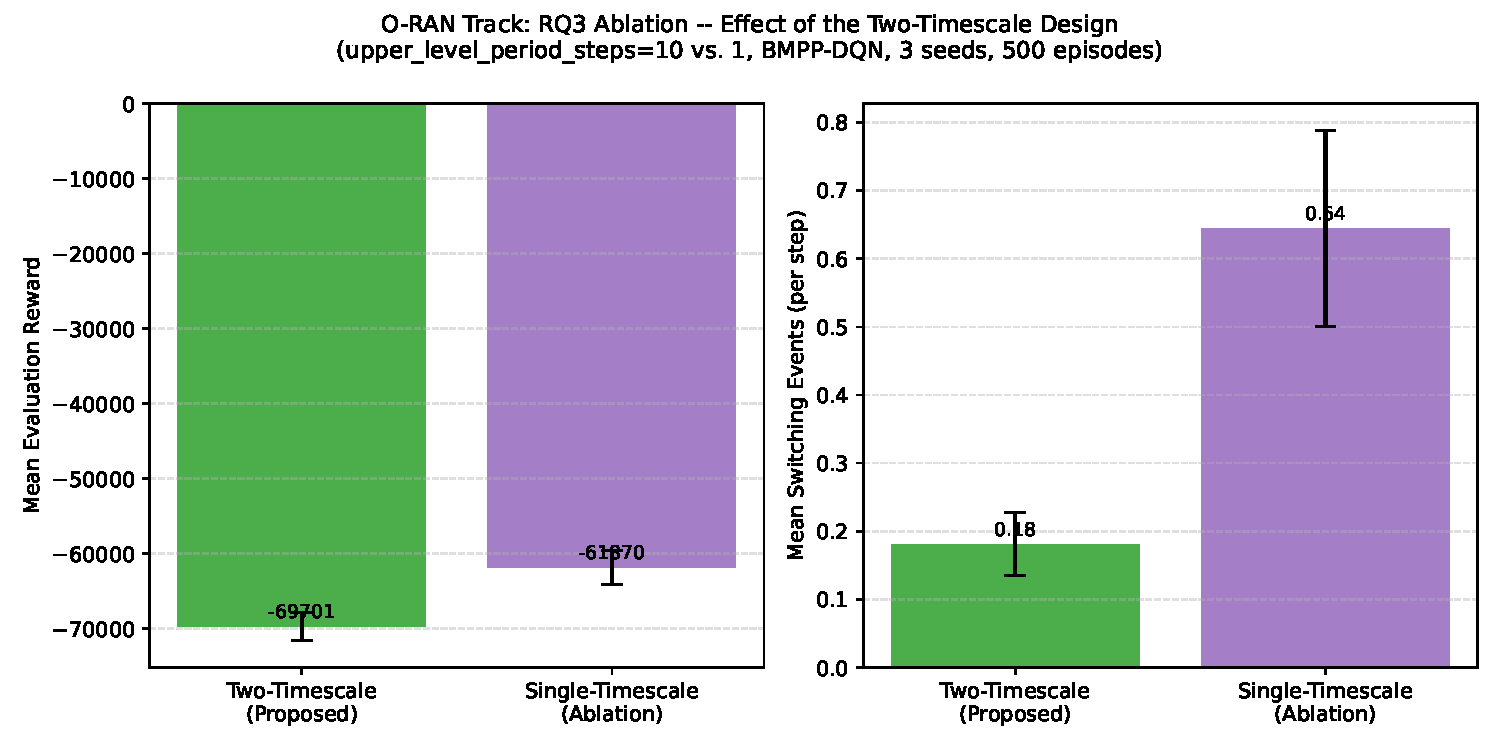
\includegraphics[width=0.8\textwidth]{../figures_oran/rq3_ablation_oran.pdf}
\caption{Reward and switching frequency: two-timescale (proposed, $N=10$)
  vs.\ single-timescale ($N=1$) BMPP-DQN, mean across 3 seeds.}
\label{fig:oran-rq3}
\end{figure}

Collapsing to a single timescale yields a mean reward of $-65251.9$ --
\emph{better} (less negative) than the two-timescale default's
$n=10$ canonical $-79443.7$ -- with higher mean power
($178.3\,\mathrm{W}$ vs.\ $154.4\,\mathrm{W}$) and higher throughput
($214.0$ vs.\ $162.6\,\mathrm{Mbps}$); QoS is comparable ($21.2\%/77.0\%$
vs.\ $20.2\%/75.8\%$). As in the earlier $n=3$-canonical version of this
chapter, the two configurations are \emph{not} reward/power-neutral: the
single-timescale variant achieves better reward by spending more power, a
genuine trade-off, not a free difference.

Switching frequency still separates the two designs sharply: the
single-timescale variant's mean switching frequency is $0.948$
events/step -- $4.5\times$ the two-timescale default's $0.211$, with no
per-seed overlap (Appendix~\ref{sec:oran-appendix-perseed-rq3}: every
single-timescale seed, lowest $0.684$, exceeds every two-timescale seed,
highest $0.251$ -- the single-timescale variant's own seed set stayed at
$n=3$, so this compares 3 seeds against the $n=10$ canonical set's own
10).

This answers RQ3, with a more qualified conclusion than the pre-fix
chapter reported: \textbf{the two-timescale design substantially reduces
switching frequency, but this now comes at a measurable cost in reward
and power, not for free.} Holding discrete RU-activation and
split-selection decisions fixed for $N=10$ steps at a time trades some
reward/throughput for decision stability -- a trade-off consistent with
Non-RT RIC decisions being intended to operate on a slower cadence than
Near-RT RIC decisions (Section~\ref{sec:oran-background}), but one this
thesis can no longer describe as costless.

\section{Inference-Time Latency}
\label{sec:oran-latency}

\begin{figure}[htbp]
\centering
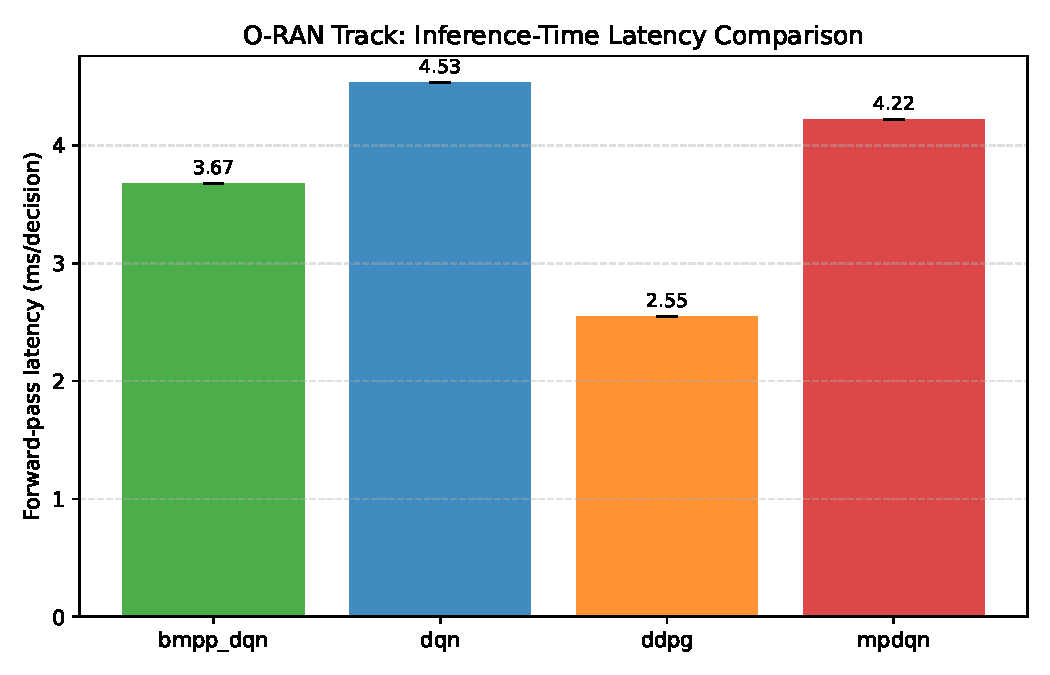
\includegraphics[width=0.6\textwidth]{../figures_oran/latency_benchmark_oran.pdf}
\caption{Per-decision forward-pass latency (ms/decision) for all 4 methods
  at this track's single default scenario ($R=4$), averaged over repeated
  greedy action selections on the same evaluation hardware.}
\label{fig:oran-latency}
\end{figure}

Consistent with this track's focused single-gNB scope
(Section~\ref{sec:oran-scope}), this benchmark measures forward-pass
latency at the one default scenario rather than across a range of network
sizes (contrast the C-RAN track's $R=5$-to-$50$ scalability sweep).
Measured latencies are $5.05\,\mathrm{ms}$ (BMPP-DQN), $5.23\,\mathrm{ms}$
(DQN), $3.24\,\mathrm{ms}$ (DDPG), and $5.57\,\mathrm{ms}$ (MP-DQN) per
decision. All four methods are small feedforward networks (hidden sizes
$[128,64]$, Section~\ref{sec:oran-bmpp-architecture}) evaluated on the
same hardware; BMPP-DQN's additional architectural components relative to
the single-network baselines -- two separate encoders, a branching
critic, and a continuous parameter network, evaluated together for one
decision (Section~\ref{sec:oran-bmpp-architecture}) -- add negligible
latency in practice (within $1\,\mathrm{ms}$ of DQN/MP-DQN), and all four
remain comfortably within a single forward-pass budget on commodity
hardware, well inside the $10$--$100\,\mathrm{ms}$ Near-RT RIC decision
loop this design's lower level targets.

\section{The \texorpdfstring{$n=3\to n=10$}{n=3 to n=10} Statistical-Power Expansion}
\label{sec:oran-n10}

Every table and figure earlier in this chapter already uses the $n=10$
canonical scale this section documents -- a change from this chapter's
own earlier revision, which reported the comparison at $n=3$
(Concept Note Section 5.3's original protocol) and flagged a known
limitation: a pre-fix-environment $n=10$ check (archived at
\texttt{thesis/tables\_oran\_archive/\allowbreak pre\_env\_bugfix\_20261001/tables\_oran\_10seed/})
had found that some pairwise significance verdicts and the MCDA
robustness picture both changed between $n=3$ and $n=10$, and whether
the same held under the corrected environment was explicitly left
unanswered. This chapter now answers it directly, using the
\emph{corrected}-environment comparison at both sample sizes.

\begin{table}[h]
\centering
\caption{Paired significance of each baseline's reward against BMPP-DQN,
  corrected environment, at $n=3$ (this chapter's own earlier
  canonical scale) vs.\ $n=10$ (current canonical scale).}
\label{tab:oran-n3-vs-n10}
\begin{tabular}{lcccc}
\hline
Baseline & $p$ ($n=3$) & $d$ ($n=3$) & $p$ ($n=10$) & $d$ ($n=10$) \\
\hline
DQN & $0.015$ & $-4.65$ & $0.0056$ & $-1.14$ \\
DDPG & $0.050$ & $2.48$ & $0.631$ & $0.16$ \\
MP-DQN & $0.377$ & $-$ & $0.116$ & $-0.55$ \\
\hline
\end{tabular}
\end{table}

\textbf{Two verdicts move, in opposite directions from what the
pre-fix $n=3\to n=10$ expansion found.} DDPG's comparison was
\emph{on the edge of significance} at $n=3$ ($p=0.050$) and is now
\textbf{solidly non-significant} at $n=10$ ($p=0.631$) -- the reverse of
the pre-fix pattern, where DDPG's deficit \emph{became} significant with
more seeds. DQN's comparison stays significant at both sample sizes, but
its effect size collapses by more than $4\times$ ($d=-4.65 \to -1.14$),
consistent with the $n=3$ estimate being substantially inflated by
small-sample variance rather than describing a stable large effect.
MP-DQN's comparison was and remains non-significant. The direction these
verdicts move is not predictable from the pre-fix pattern -- more seeds
changed the picture again, but not by repeating what more seeds did
before.

The MCDA robustness picture shows the same kind of instability.
Section~\ref{sec:oran-mcda-robustness}'s $n=10$ finding -- BMPP-DQN
ranks \#2 under both TOPSIS variants but \#4 (worst of four) under VIKOR
-- is a more dramatic reversal than the pre-fix $n=3\to n=10$ expansion
found (there, BMPP-DQN stayed rank 1-or-2 under every scheme at both
sample sizes, just losing perfect three-way agreement). \textbf{The
practical lesson is the same either way: this track's $n=3$ protocol is
not a reliable basis for either a significance claim or a multi-criteria
ranking claim}, and every comparison in this chapter should be read at
its $n=10$ sample size, not the $n=3$ figures an earlier revision of
this chapter reported.

\section{Discussion: Answering the Research Questions}
\label{sec:oran-rq-answers}

\textbf{RQ1} (architectural integration, Section~\ref{sec:oran-research-questions}):
BMPP-DQN trains stably end-to-end as a single coupled network combining
branching discrete decomposition with multi-pass continuous parameter
processing (Chapter~\ref{chap:oran-system-model}), across all 10 seeds,
with no divergence or training-instability failures observed, under the
corrected environment and algorithm (Section~\ref{sec:oran-bugfixes}).
This is an architectural and training-stability claim, evidenced by the
convergence behavior in Section~\ref{sec:oran-convergence} and the
consistent final performance across seeds in
Table~\ref{tab:oran-convergence}; it does not by itself establish that
the architecture integrates its two halves \emph{efficiently}, which
Section~\ref{sec:oran-calibration}'s finding (a simple heuristic beats
BMPP-DQN's reward) weighs against.

\textbf{RQ2} (energy-saving performance): the evidence does not support a
single-metric energy-saving win, and does so more starkly than the
pre-fix chapter found. BMPP-DQN's reward is significantly \emph{worse}
than DQN's ($p=0.0056$ at $n=10$), and both a trivial heuristic and a
privileged oracle significantly beat every trained method's reward,
BMPP-DQN included (Section~\ref{sec:oran-calibration}). Objective 4's
$\geq15\%$ energy-saving target against the trained baselines is, without
qualification, \textbf{not met} by any result in this chapter -- and the
calibration check now shows the gap is not merely "no baseline beats
BMPP-DQN by $15\%$," but "an untrained rule beats every trained method
including BMPP-DQN at all." The multi-criteria-balance claim this
chapter's $n=3$ version made -- BMPP-DQN ranks first-or-second under
every MCDA scheme, the only method with that consistency -- \textbf{does
not survive the $n=10$ revalidation}: BMPP-DQN still ranks \#2 under both
TOPSIS variants, but \#4 (worst of four) under VIKOR
(Section~\ref{sec:oran-mcda-robustness}), and no method agrees across all
three schemes at this sample size. What remains defensible is narrower:
BMPP-DQN ranks \#2 of 4 under two of the three independent schemes tested
(both TOPSIS variants, which agree with each other exactly), not under
every scheme, and the honest reading is that this track's earlier
multi-criteria-robustness claim was itself an $n=3$-sample artifact
(Section~\ref{sec:oran-n10}). Section~\ref{sec:oran-cadence-control}'s
fair-cadence control further qualifies the switching-frequency input to
this ranking: BMPP-DQN's switching-frequency advantage over DQN/MP-DQN at
their own default cadence is substantially a cadence artifact, not an
architectural one -- at matched cadence, both baselines switch
\emph{less} than BMPP-DQN, with no offsetting reward cost at the $n=10$
canonical sample size either.

\textbf{RQ3} (two-timescale design): directly answered in
Section~\ref{sec:oran-rq3}. Collapsing the two-timescale separation to a
single timescale reduces switching stability by $4.5\times$ but
\emph{improves} reward and throughput at the cost of higher power -- a
genuine trade-off, not the previously-reported free reduction in
switching. The two-timescale design's contribution is decision stability
at the discrete-action level, purchased at a measurable reward/power
cost, matched to the Non-RT/Near-RT RIC timescale separation this problem
is built on (Section~\ref{sec:oran-background}).

Chapter~\ref{chap:oran-conclusion} returns to these three answers,
including the honest reconciliation Section~\ref{sec:oran-calibration}
and Section~\ref{sec:oran-cadence-control} now require, alongside this
thesis's scope and limitations (Section~\ref{sec:oran-scope}) to state
its overall contribution and directions for future work.

% ---------------------------------------------------------------------------
% This chapter's citations (hwang1981topsis, zeleny1982mcdm,
% opricovic2004vikor, cohen1988statistical) resolve against the
% consolidated thesis-wide bibliography in
% thesis/chapters/references_oran.tex, not a local thebibliography here.
% ---------------------------------------------------------------------------
